%\documentclass[aspectratio=10]{beamer} %For normal presentation (comment otherwise)
\documentclass[aspectratio=169]{beamer} %for widescreen prestentation
\usetheme{default}%{Singapore}
\usefonttheme{serif}
\usepackage{ulem}
\usecolortheme{default}%albatross, crane, beetle, dove, fly, seagull, wolverine e beaver.
\setbeamertemplate{frametitle}[default][center]
%%%%%%%%%%%%%%%%%%%%%%%%%%%%%%%%%%%%%%%%%%%%%%%%%%%%%%%%%%%%%%%%%%%%%%%%%%%%%%%%%%%%%%%%%%%%%%%
%%%%%%%%%%%%%%%%%%%%%%%%%%%%%%%%%%%%%%EXTRA PACTAGES%%%%%%%%%%%%%%%%%%%%%%%%%%%%%%%%%%%%%%%%%%%
\usepackage[utf8]{inputenc}
\usepackage[T1]{fontenc}
\usepackage[scaled]{helvet}
\renewcommand*\familydefault{\sfdefault}
\usepackage[portuguese, english]{babel}
\usepackage[round]{natbib}
\usepackage{hyperref} 
\usepackage{tcolorbox}
\usepackage{graphicx} % Required for including images
\usepackage{graphics}
%\usepackage[dvips]{graphicx} 
\graphicspath{{images/}} % Location of the graphics files
\usepackage{booktabs} % Top and bottom rules for table
\usepackage[font=small,labelfont=bf]{caption}%specifies captions on tables and figures
\usepackage{amsfonts, amsmath, amsthm, amssymb} % For math fonts, symbols and environments
\usepackage{wrapfig} % Allows wrapping text around tables and figures
\usepackage{makeidx}
\usepackage{epstopdf}%adiciona images em formato eps no pdf.
\usepackage{subfigure}%cria ambientes de multifiguras
\usepackage{float}%coloca as figuras exatamente aonde você quer
\usepackage{times}
\usepackage{tikz}%pacote para fazer fluxogramas
\usepackage{epsfig}
\usepackage{url}
\usepackage{xurl}
\usepackage{epstopdf} %converting to PDF
\usepackage{verbatim}%
\usepackage{multicol}
\usepackage{xcolor}
\usepackage[makeroom]{cancel}
\usepackage[framemethod=tikz]{mdframed}
\usepackage{hyperref} 
\usepackage{smartdiagram}
\usesmartdiagramlibrary{additions}
\smartdiagramset{%uniform color list=white!60!black for 6 items,
	back arrow disabled=true, module minimum width=1.8cm,
	module minimum height=2cm,
	module x sep=2.7cm,
	text width=1.8cm,
	additions={
		additional item offset=0.5cm,
		additional item width=2cm,
		additional item height=2cm,
		additional item text width=3cm
	}
}
  
\usepackage{amssymb}
\usepackage{etoolbox}
\usepackage{tikz}
\usetikzlibrary{mindmap}
\usepackage{metalogo}
%\smartdiagramset{uniform color list=gray!60!black for 6 items,
%back arrow disabled=false}
\usepackage{booktabs} % Top and bottom rules for table
\usepackage[font=small,labelfont=bf]{caption} % Required for specifying captions to 


% Configuracao das referencias
\hypersetup{
    colorlinks=true,
    citecolor=blue,   % Cor das refer\u00eancias citadas
    linkcolor=blue,   % Cor dos links
    urlcolor=blue     % Cor dos links para URLs
}

% Configurar as cita\u00e7\u00f5es com par\u00eanteses e a cor azul
\setcitestyle{round} % Par\u00eanteses ao inv\u00e9s de colchetes

% Definir cor azul para cita\u00e7\u00f5es, incluindo par\u00eanteses
%\renewcommand{\cite}[1]{\textcolor{blue}{\citet{#1}}}
%\renewcommand{\citep}[1]{\textcolor{blue}{\citep{#1}}}

%%%%%%%%%%%%%%%%%%%%%%%%%%%%%%%%%%%%%%%%%%%%%%%%%%%%%%%%%%%%%%%%%%%%%%%%%%%%%%%%%%%%%%%%%%%%%
%%%%%%%%%%%%%%%%%%%%%%%%%%%%%%%%%%%%% PREAMBLE %%%%%%%%%%%%%%%%%%%%%%%%%%%%%%%%%%%%%%%%%%%%%%%%
%\subtitle{}
\author[Victor Carreira]{} 
\title{A inteligência artificial é inteligente?}
\subtitle{Hunger of Science}
\institute{LOOP}
\date{Setembro de 2024}
\subject{Grupo LOOP}
%\setbeamertemplate{footline}[frame number]
%\setbeamercovered{transparent}
\setbeamertemplate{navigation symbols}{}
% Tela cheia
\hypersetup{pdfpagemode=FullScreen}
\usepackage{ragged2e}
%\justifying
%\addtobeamertemplate{headline}{}
\usepackage{tikz}
\usetikzlibrary{shapes.geometric, arrows}

% Criar um novo comando para destacar o primeiro item
\patchcmd{\sectioninToC}{\inserttocsection}{\ifnumequal{\inserttocsectionnumber}{1}{\textbf{\inserttocsection}}{\inserttocsection}}{}{}


%%%%%%%%%%%%%%%%%%%%%%%%%%%%%%%%%%%%%%%%%%%%%% PRESENTATION %%%%%%%%%%%%%%%%%%%%%%%%%%%%%%%%%%%%%%%%%%%%%%%
\begin{document}


\bgroup
\makeatletter
\setbeamertemplate{footline}
\makeatother
%\maketitle
\egroup
\scriptsize 
\addtobeamertemplate{navigation symbols}{}{\hskip6pt\raisebox{2pt}{\color{blue}\insertframenumber}}
\setcounter{framenumber}{0}
%\AtBeginSection[]


%%% Preambulo

%%% capa
{
\usebackgroundtemplate{
\centering
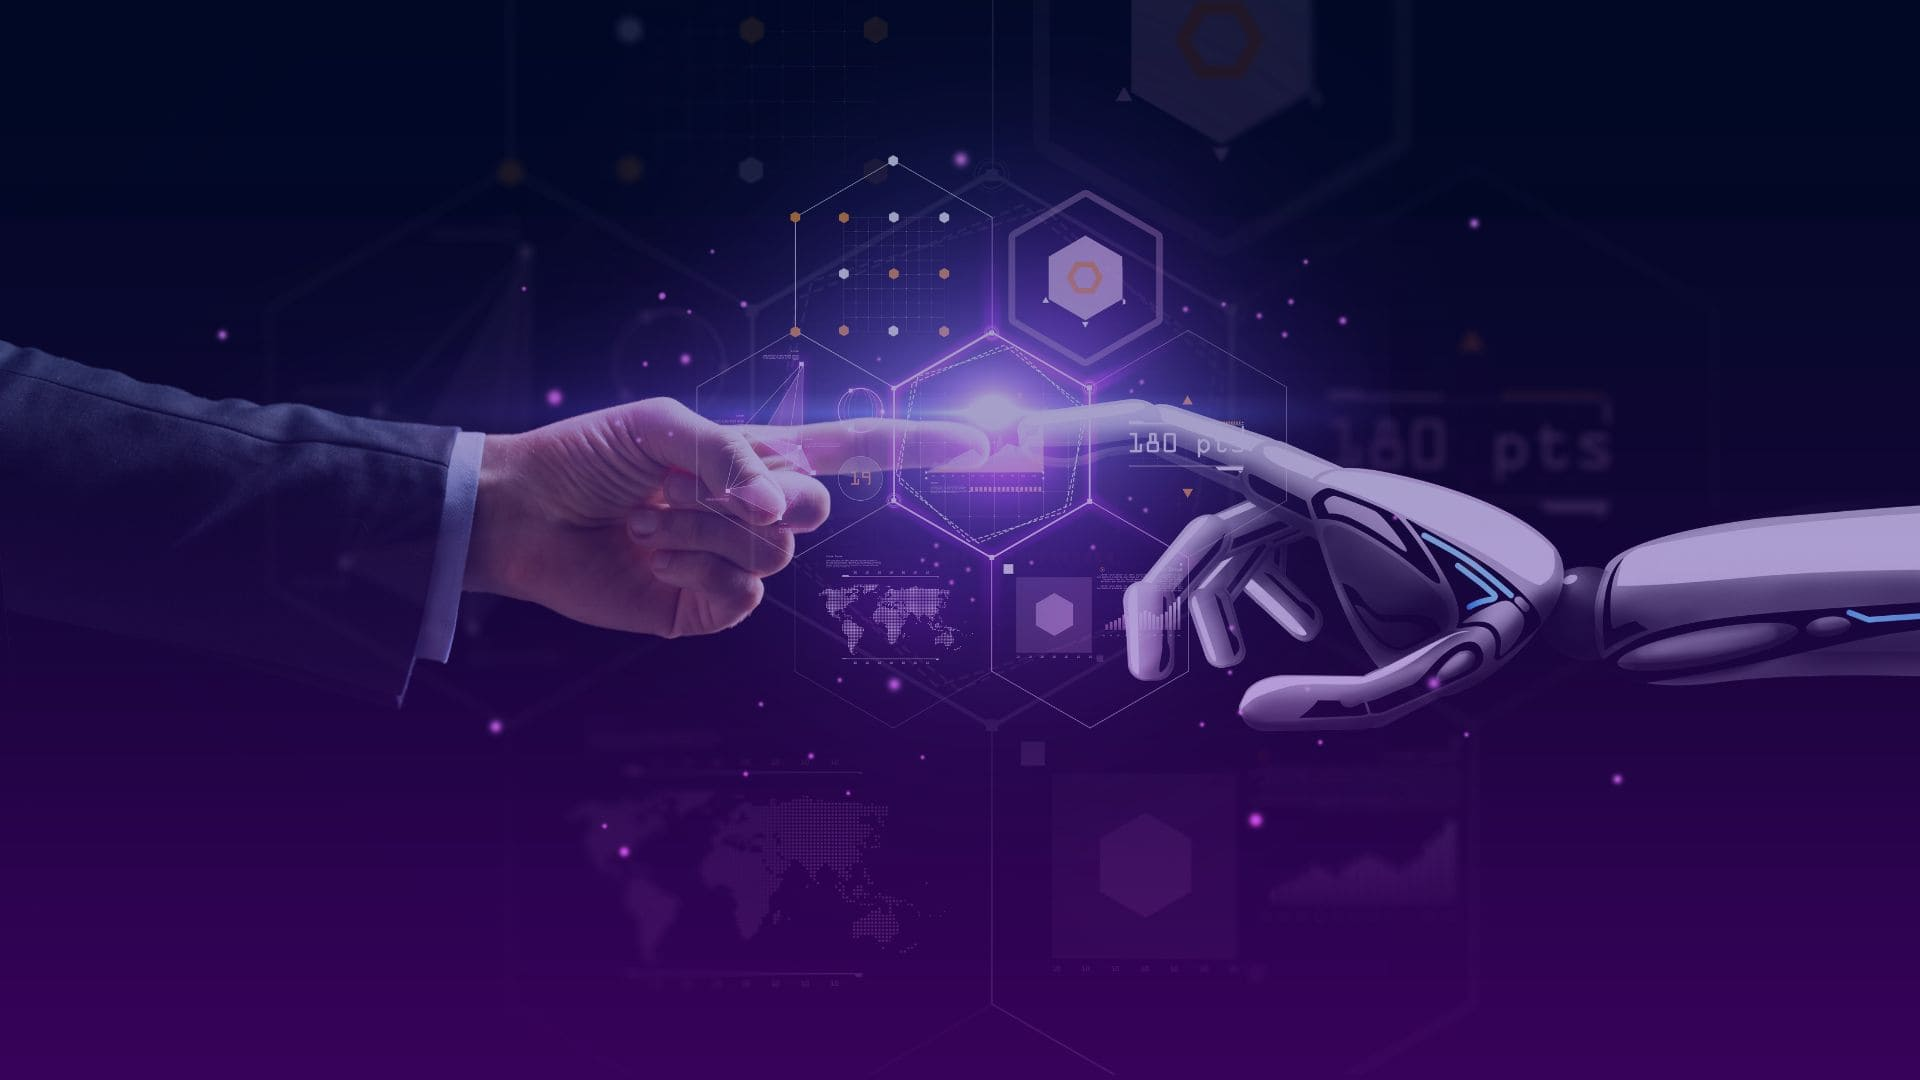
\includegraphics[width=\paperwidth,height=\paperheight]{images/capa.jpg}
}
	

\begin{frame}

\end{frame}
}


%% Titulo

{
\usebackgroundtemplate{
\centering

\includegraphics[width=\paperwidth,height=\paperheight]{images/fundo.pdf}
}
	
% Frame 3: plano de fundo
\begin{frame}
\maketitle
	
\end{frame}
}

{
\usebackgroundtemplate{
\centering

\includegraphics[width=\paperwidth,height=\paperheight]{images/fundo.pdf}
}

\begin{frame}
	\centering
	\frametitle{\textcolor{blue}{Sumário}}
    %\large
	\setbeamercolor{section in toc}{fg=blue,bg=blue}
    \tableofcontents[currentsection,sectionstyle=show/shaded,subsectionstyle=show/show/shaded]
\end{frame}

}








\section{Introdu\c{c}ão} 

{
	\usebackgroundtemplate{
		\centering
		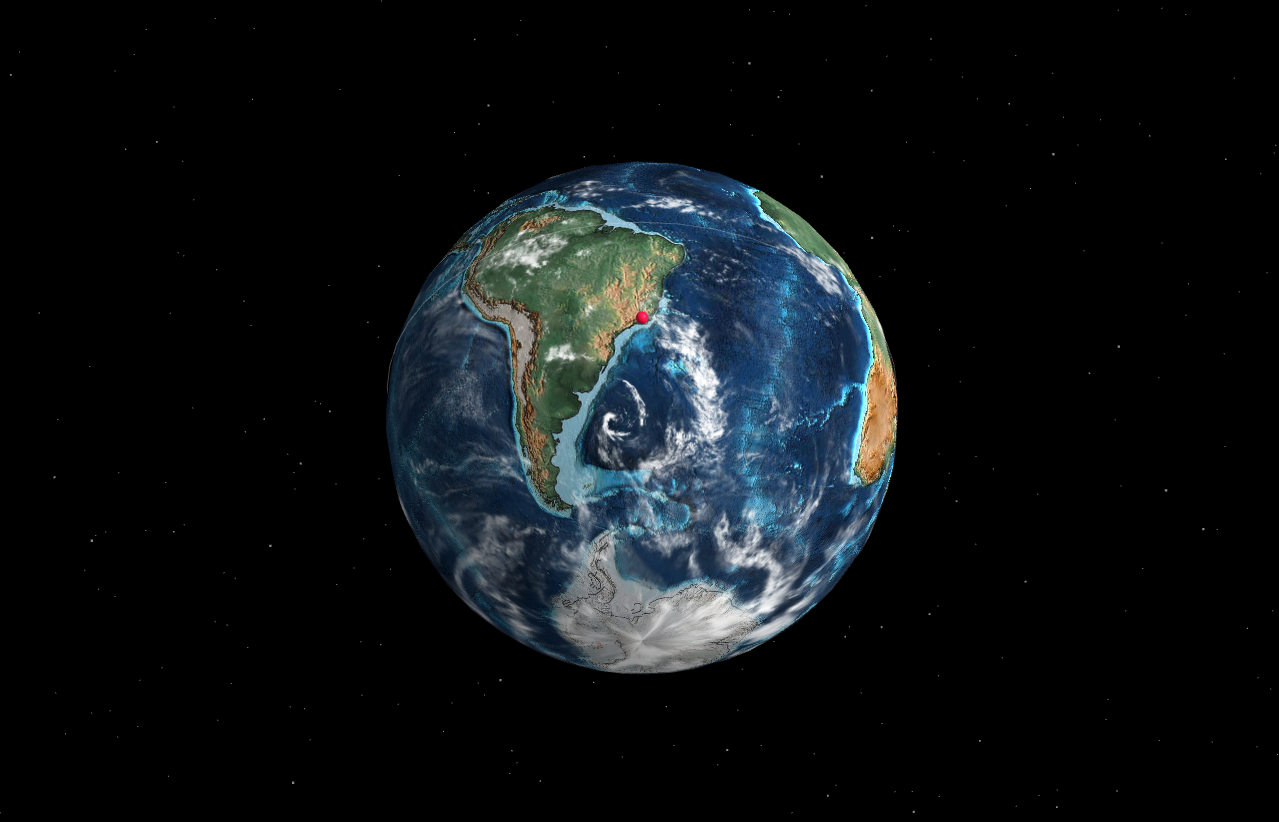
\includegraphics[width=\paperwidth,height=\paperheight]{images/holoceno.png}
	}
	
	% Frame 3: plano de fundo
	\begin{frame}
		\frametitle{\textcolor{yellow}{Olhemos para a Terra através de outra perspectiva...}}
\transboxin		


\flushright
\textcolor{yellow}{Tempo recente}
	\end{frame}
}


{
	\usebackgroundtemplate{
		\centering
		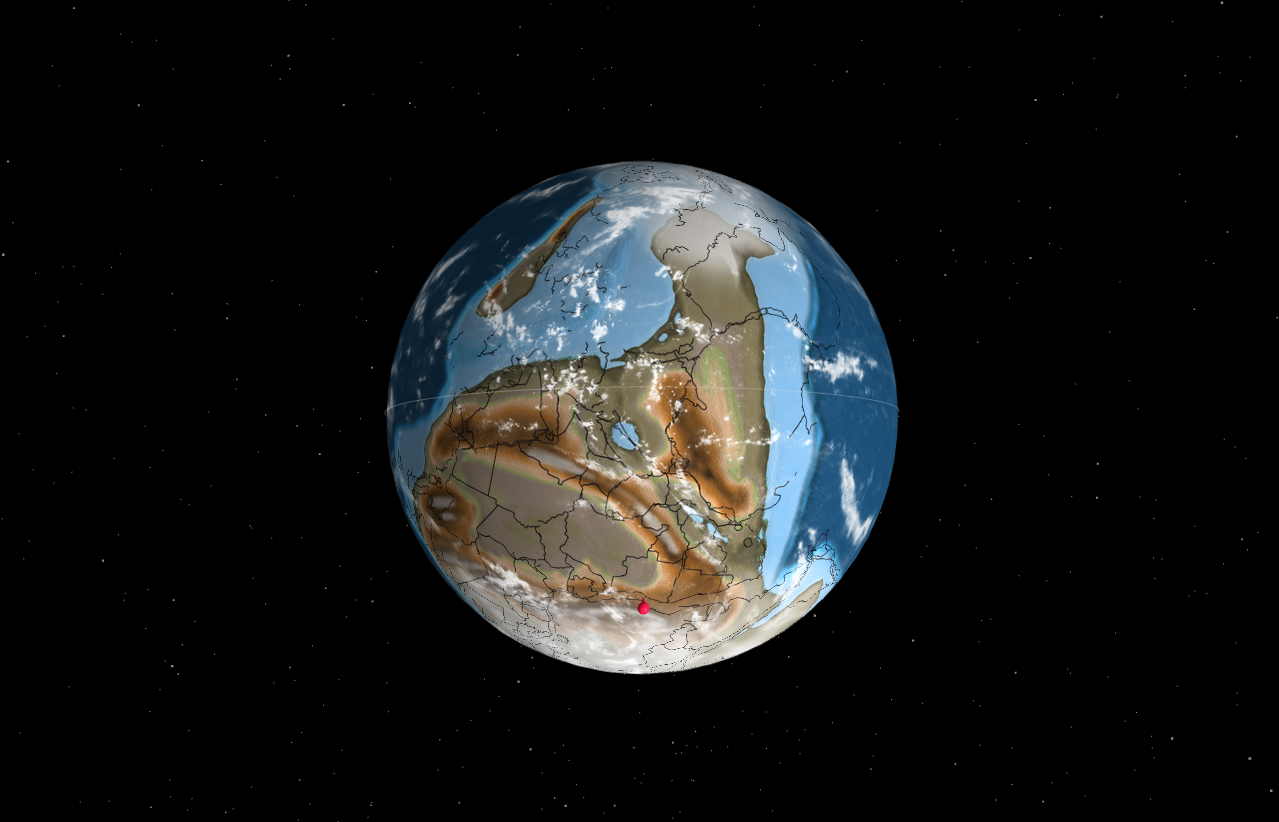
\includegraphics[width=\paperwidth,height=\paperheight]{images/ediacariano.png}
	}
	
	% Frame 3: plano de fundo
	\begin{frame}
		\frametitle{\textcolor{yellow}{E voltemos um pouco ao passado, no Ediacarano...}}
\transboxout	

\flushright
\textcolor{yellow}{$\pm$575 Ma atrás}
	\end{frame}
}


{
	\usebackgroundtemplate{
		\centering
		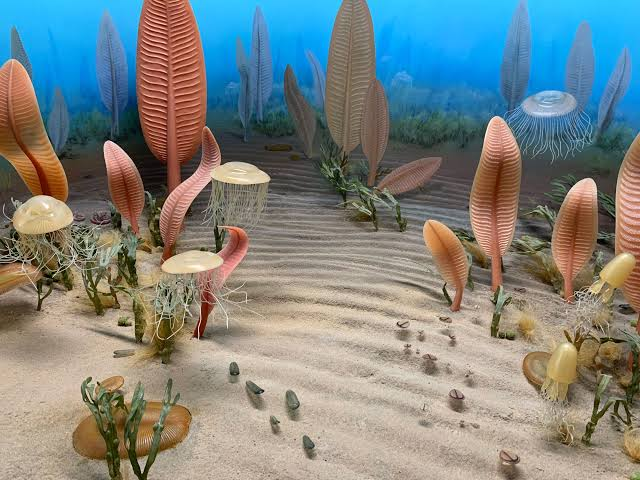
\includegraphics[width=\paperwidth,height=\paperheight]{images/faunaediacarana.jpeg}
	}
	
	% Frame 3: plano de fundo
	\begin{frame}
		\frametitle{\textcolor{yellow}{A vida diversifica-se nos oceanos}}
	\transdissolve	
	\end{frame}
}

{
	\usebackgroundtemplate{
		\centering
		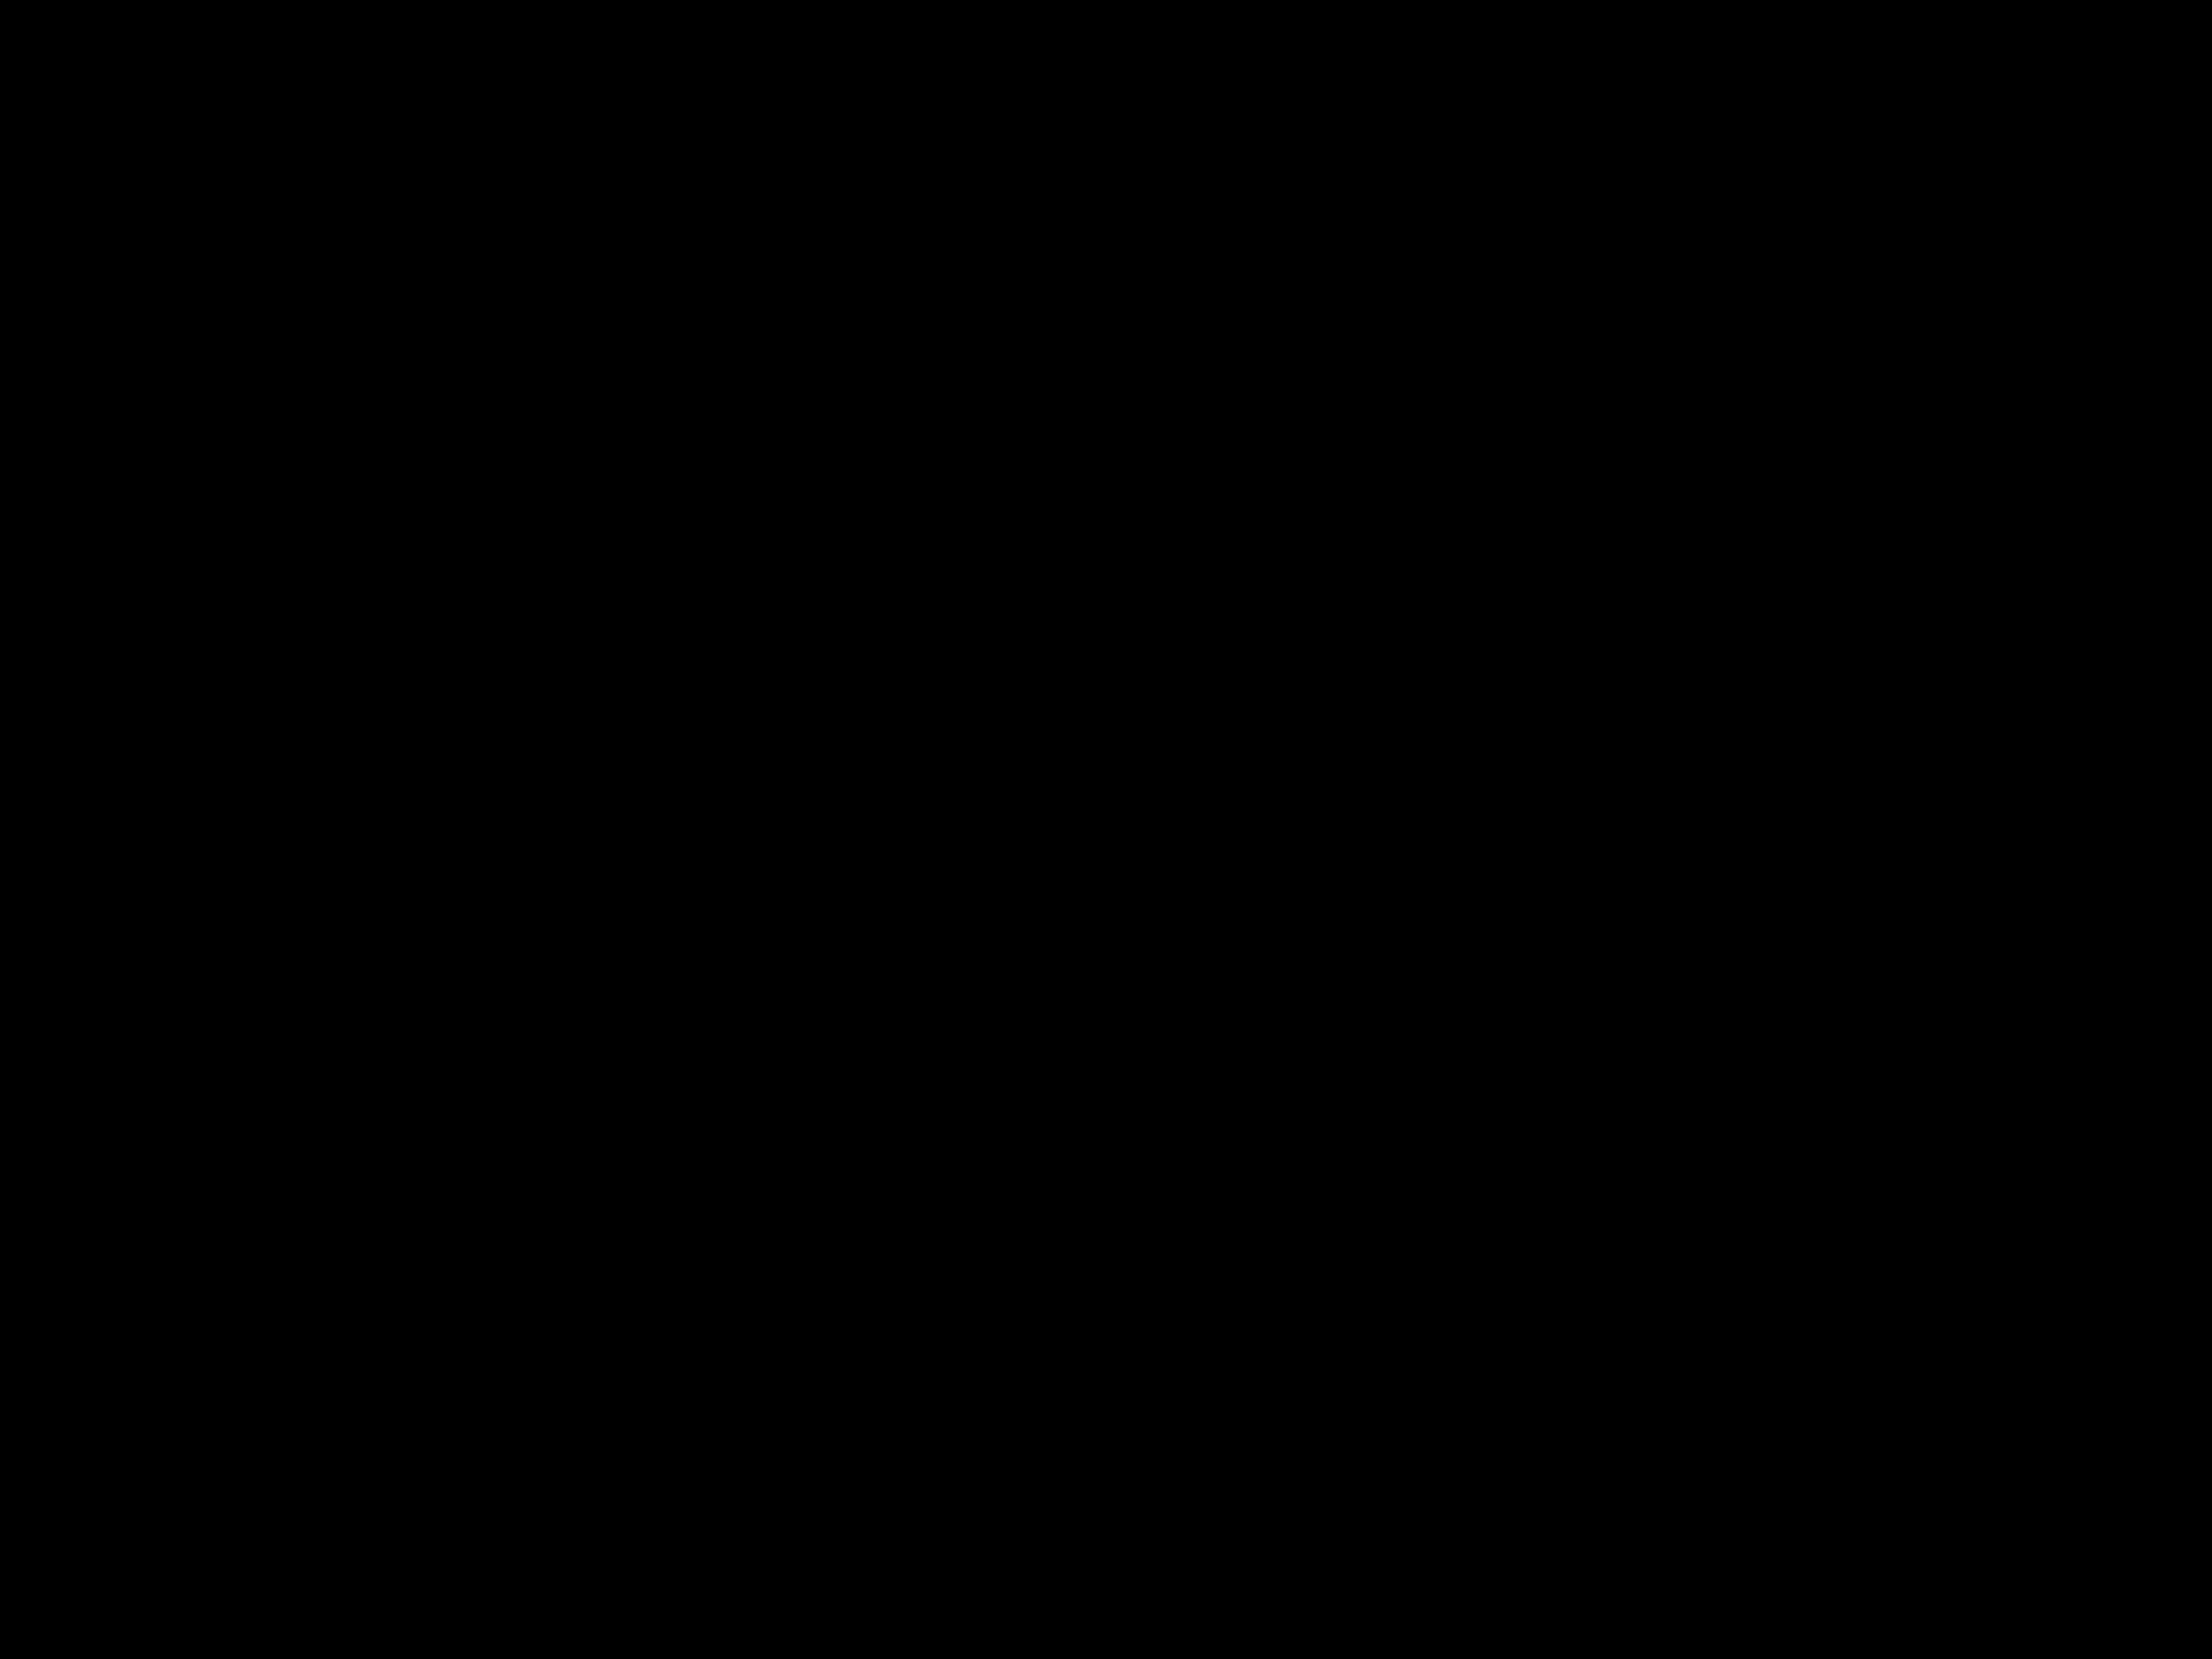
\includegraphics[width=\paperwidth,height=\paperheight]{images/fundopreto.png}
	}
	
	% Frame 3: plano de fundo
	\begin{frame}
		\frametitle{\textcolor{yellow}{Registros da Fauna de Ediacara}}
	\transboxout	
    
    \begin{minipage}{0.5\textwidth}
	    \begin{figure}
	\centering
        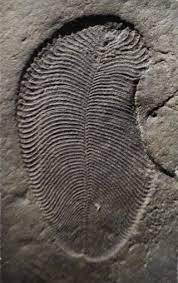
\includegraphics[scale=0.3]{images/faunaediacara3.jpeg} % Substitua pelo caminho da sua primeira figura
		    \caption{\textcolor{white}{\textit{Dickinsonia costata}, é um dos registros fósseis mais comum desse tempo.}} % Opcional
	    \end{figure}
    \end{minipage}%
		\pause
    \begin{minipage}{0.5\textwidth}
	    \begin{figure}
        \centering
        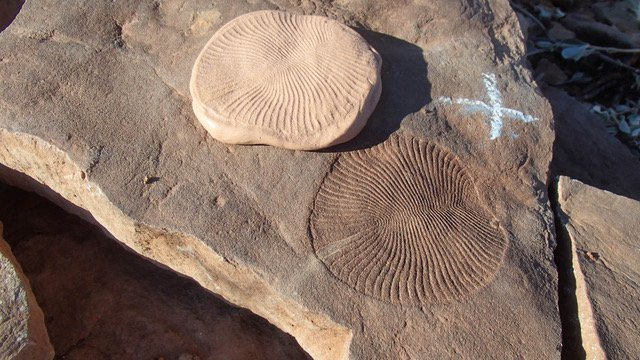
\includegraphics[scale=0.25]{images/faunaediacaran2.jpg} % Substitua pelo caminho da sua segunda figura
		    \caption{\textcolor{white}{Deslocava-se entre o sedimento de fundo, geralmente areias finas. Este espécime tinha cerca  de 6 centímetros de diâmtetro e fora encontrado, no sul da Austrália, e se alimentavam de tapetes microbialinos.}} % Opcional
	    \end{figure}
    \end{minipage}

\flushright
		\textcolor{blue}{\citep{Droser2024}}
		
	\end{frame}
}






{
	\usebackgroundtemplate{
		\centering
		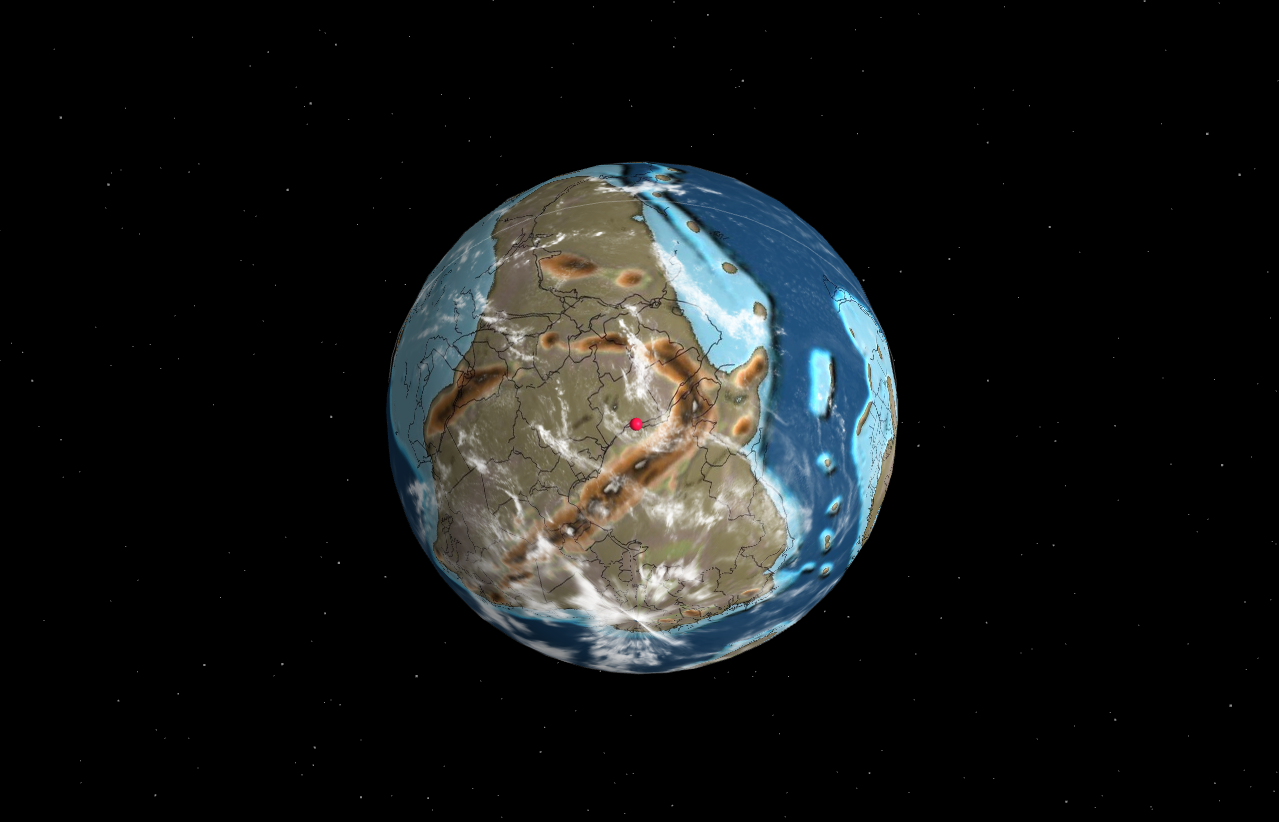
\includegraphics[width=\paperwidth,height=\paperheight]{images/cambriano.png}
	}
	
	% Frame 3: plano de fundo
	\begin{frame}
		\frametitle{\textcolor{yellow}{Avancemos um pouco mais, no tempo ...}}
	\transdissolve	
	
	\flushright
	\textcolor{yellow}{$\pm$505 Ma atrás}


\end{frame}
}




{
	\usebackgroundtemplate{
		\centering
		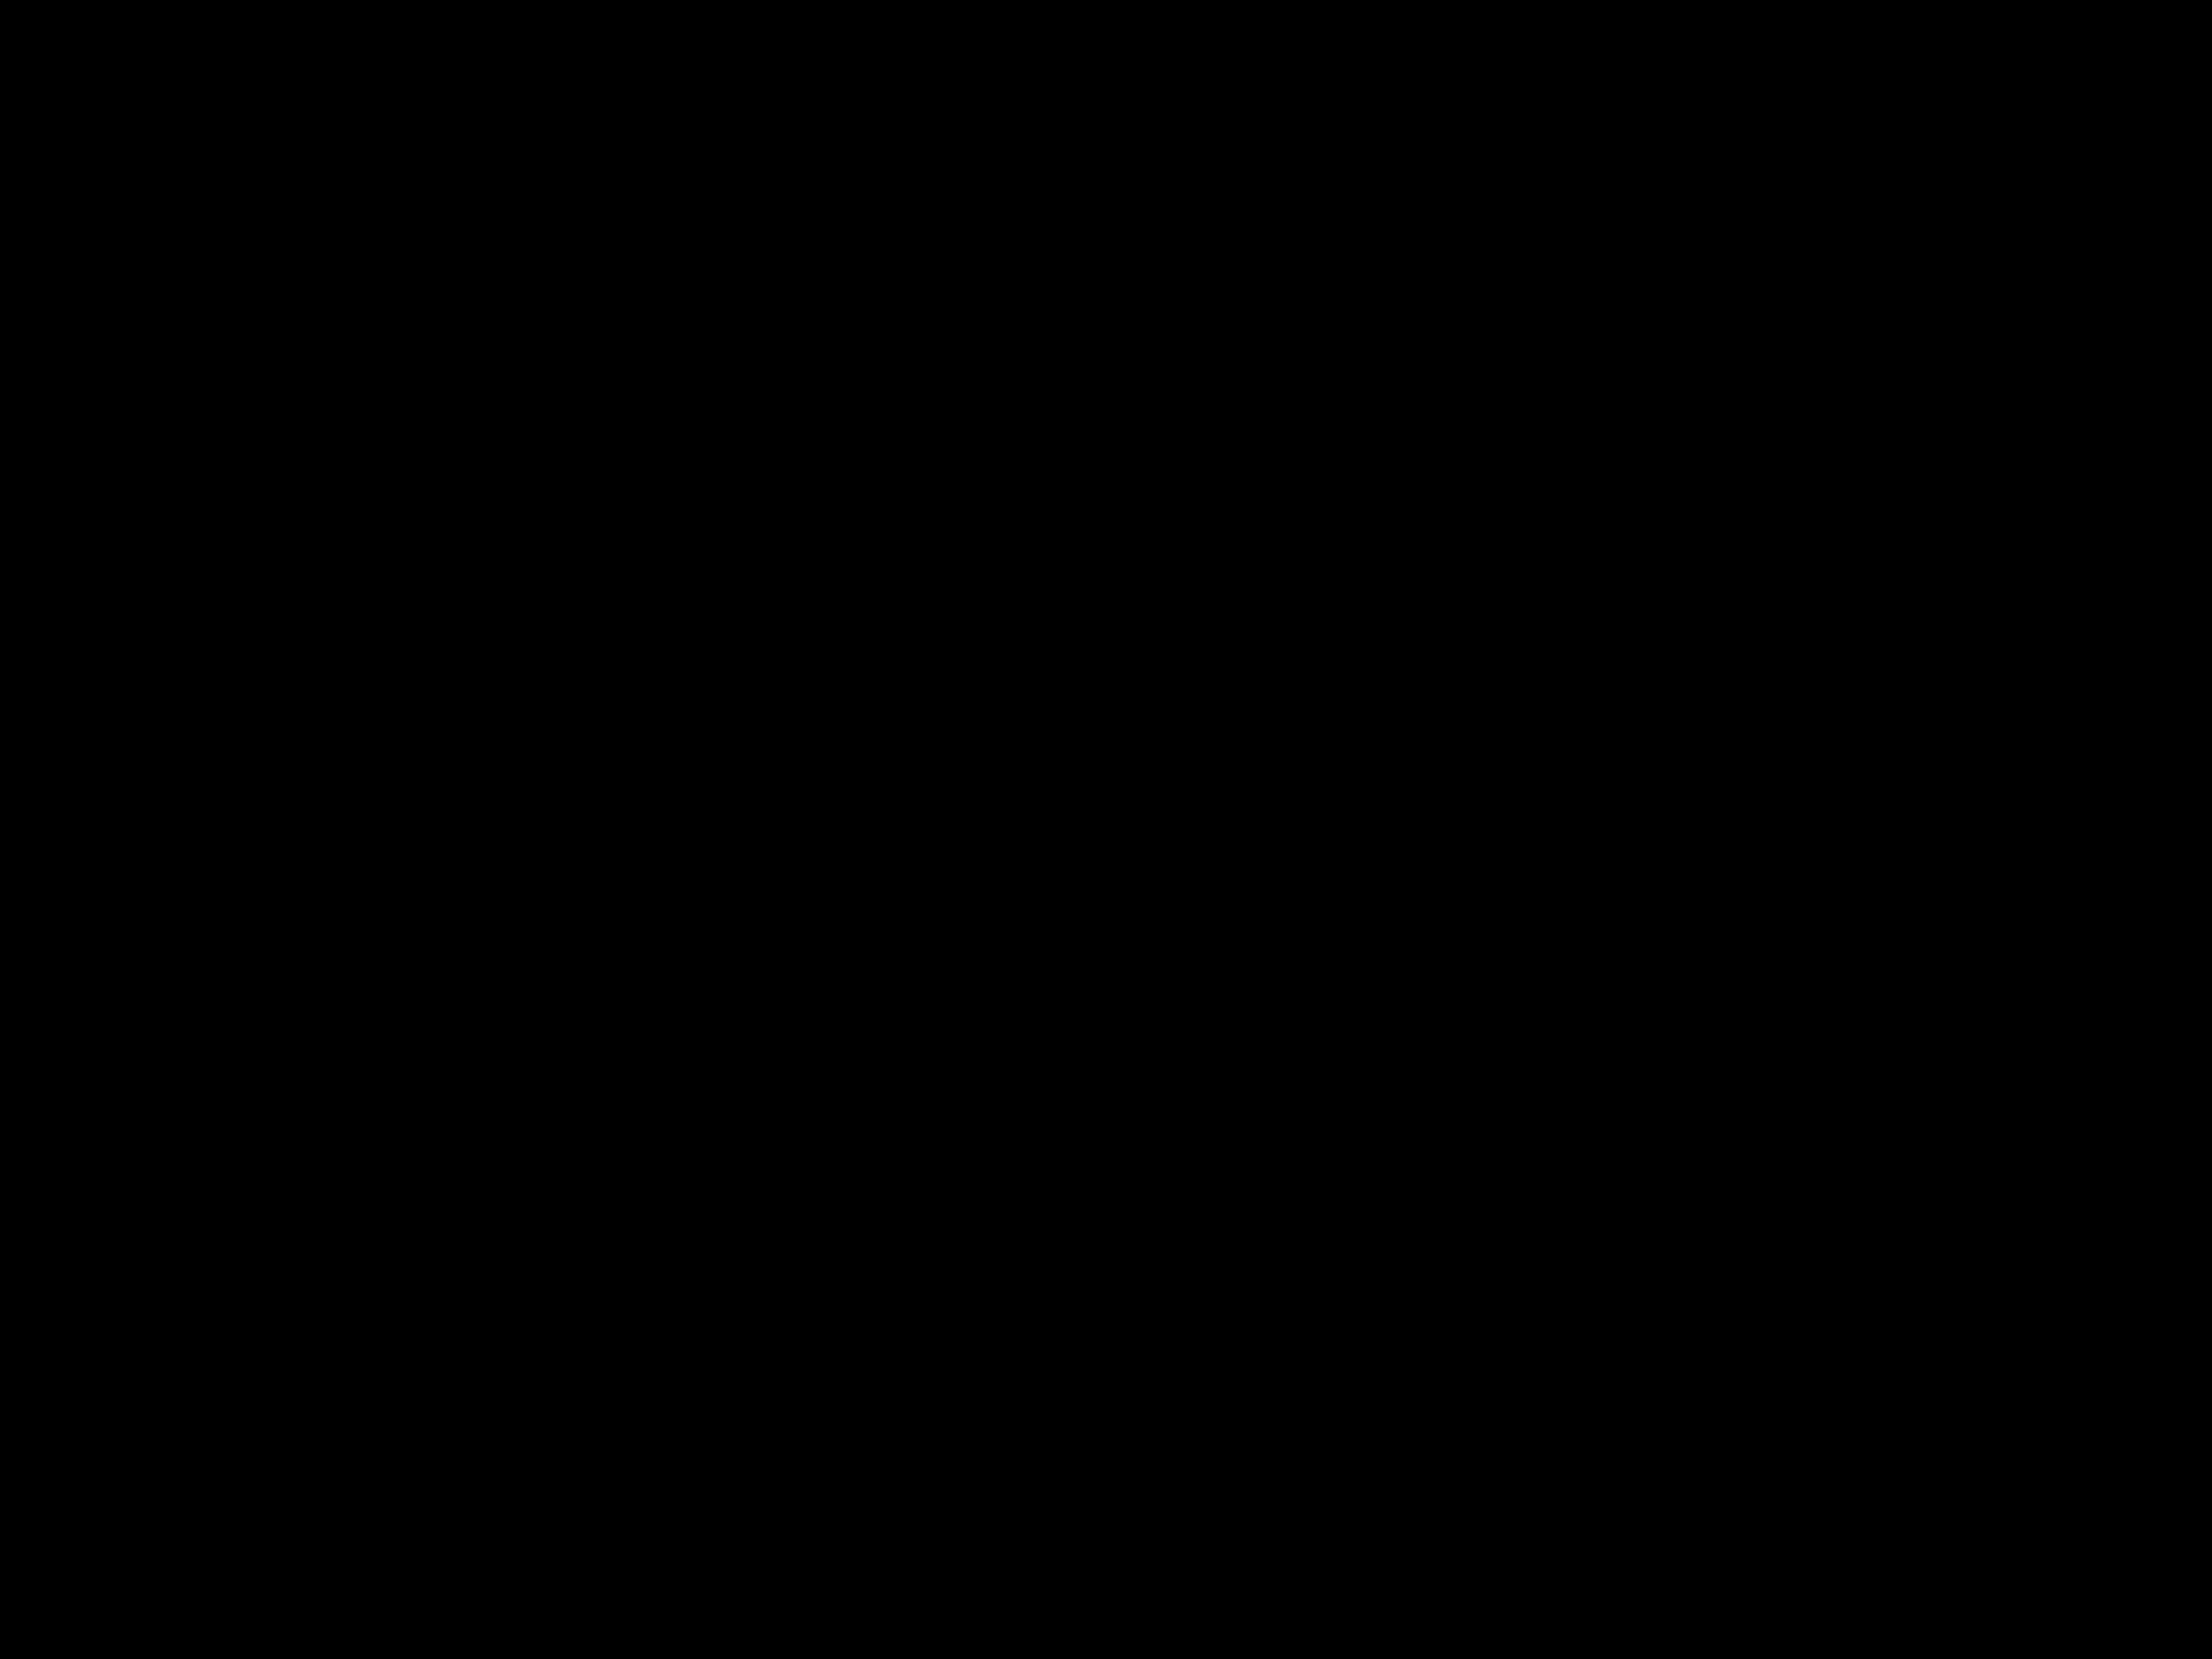
\includegraphics[width=\paperwidth,height=\paperheight]{images/fundopreto.png}
	}
	
	% Frame 3: plano de fundo
	\begin{frame}
		\frametitle{\textcolor{yellow}{Registros da Fauna de Cambriana}}
	\transboxout	
    
    \begin{minipage}{0.5\textwidth}
	    \begin{figure}
	\centering
        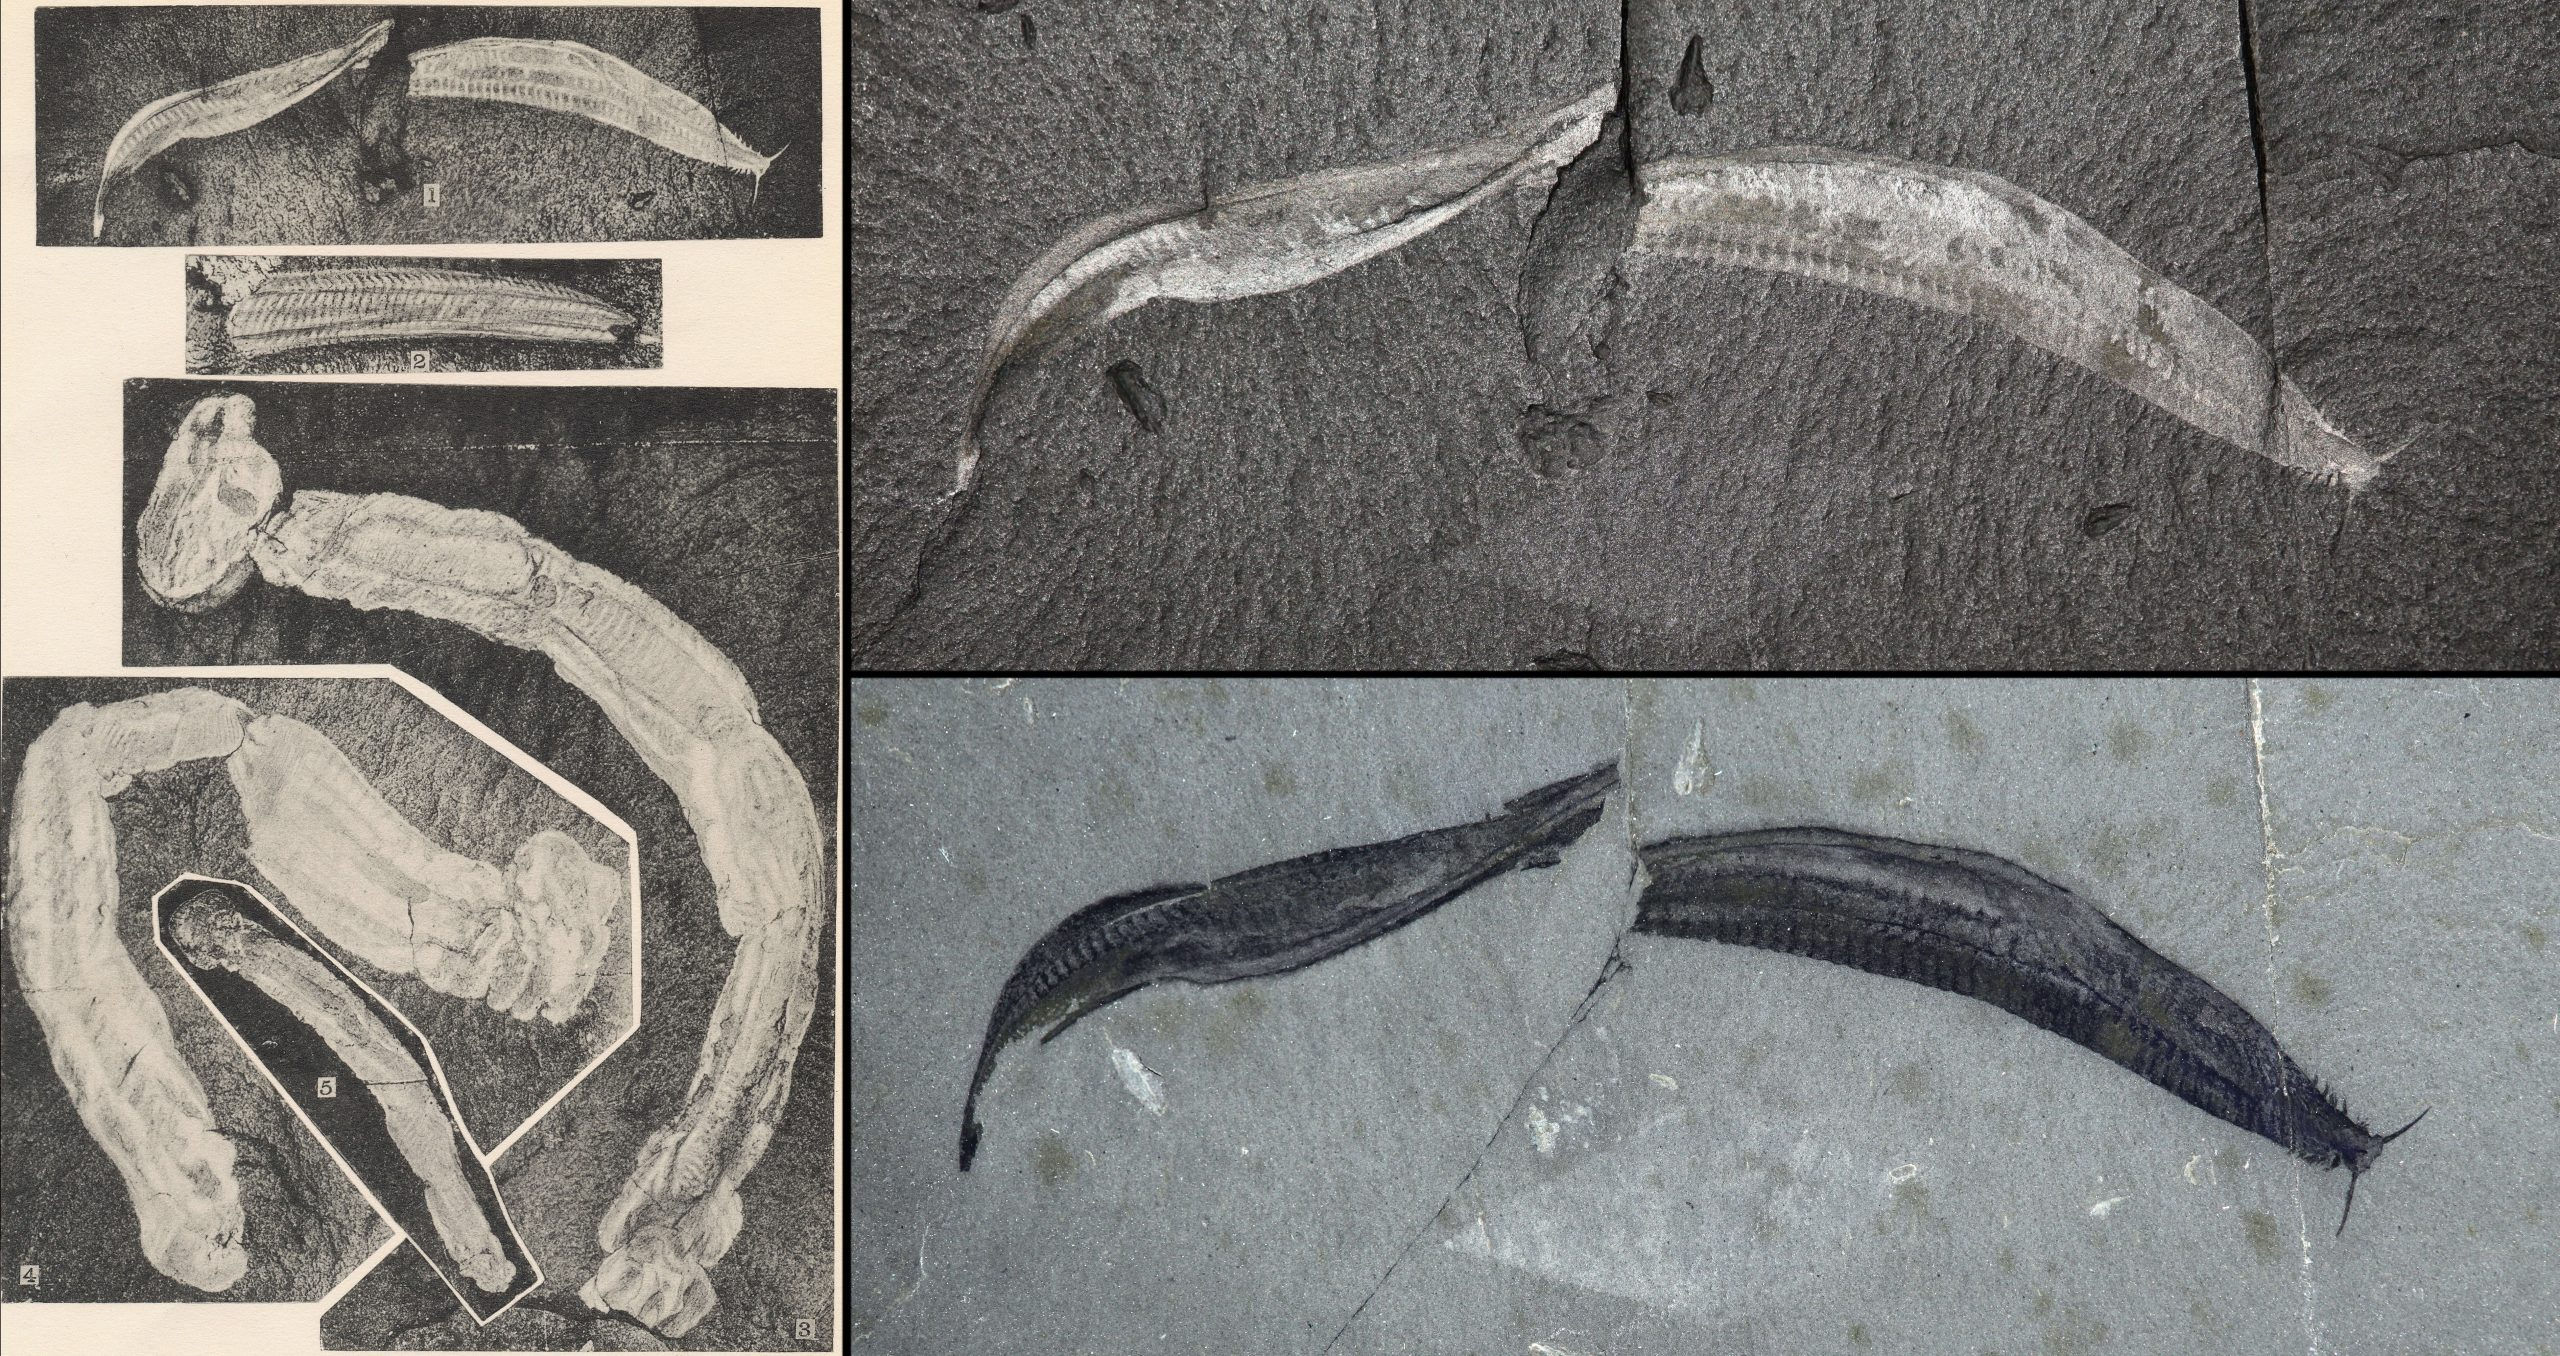
\includegraphics[scale=0.1]{images/faunacambriana3.jpg} % Substitua pelo caminho da sua primeira figura
		    \caption{\textcolor{white}{\textit{Pikaia gracilens}, é o fóssil mais notável desse tempo, representante dos primeiros cordatas com vasto registro no folhelho Burgess, no escudo Canadense.}} % Opcional
	    \end{figure}
    \end{minipage}%
		\pause
    \begin{minipage}{0.5\textwidth}
	    \begin{figure}
        \centering
        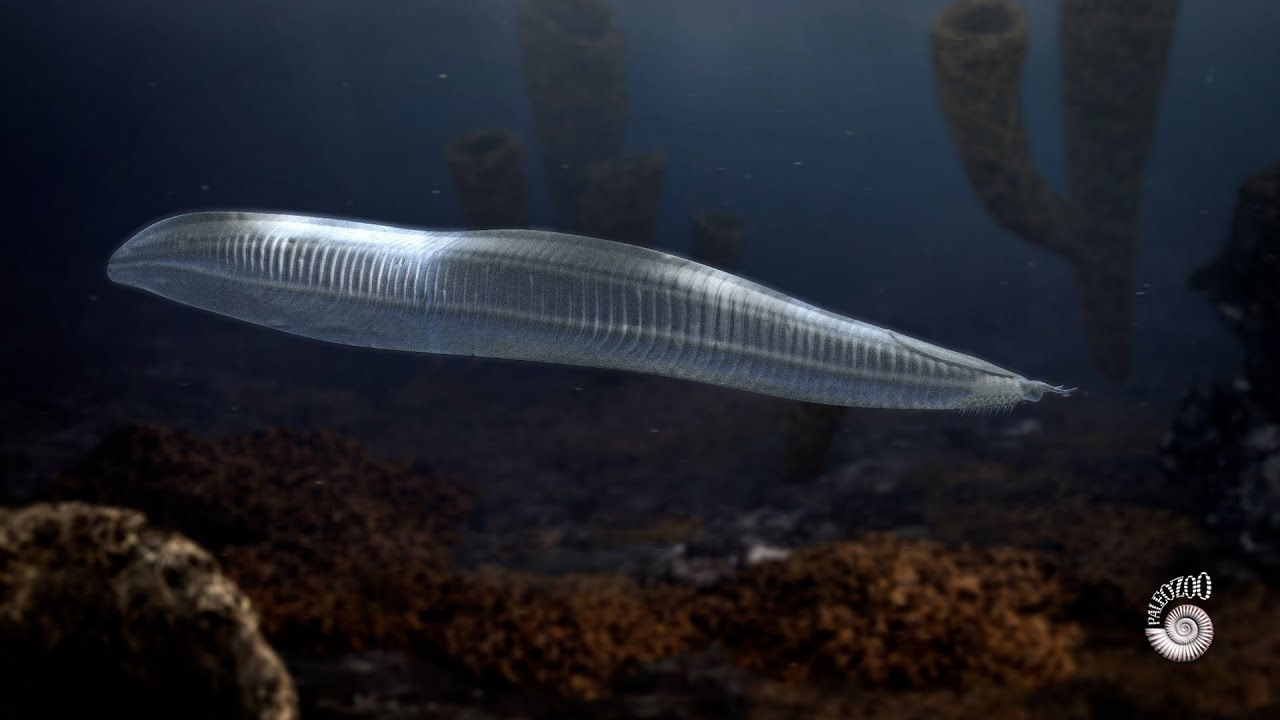
\includegraphics[scale=0.15]{images/faunacambriana2.jpg} % Substitua pelo caminho da sua segunda figura
		    \caption{\textcolor{white}{O corpo é lateralmente achatado com evidência de uma nadadeira ventral. Uma estrutura dorsal estreita que percorre o comprimento do organismo pode representar uma notocorda. Não possuem evidência de olhos.}} % Opcional
	    \end{figure}
    \end{minipage}

\flushright
		\textcolor{blue}{\citep{Briggs2015}}
		
	\end{frame}
}

{
	\usebackgroundtemplate{
		\centering
		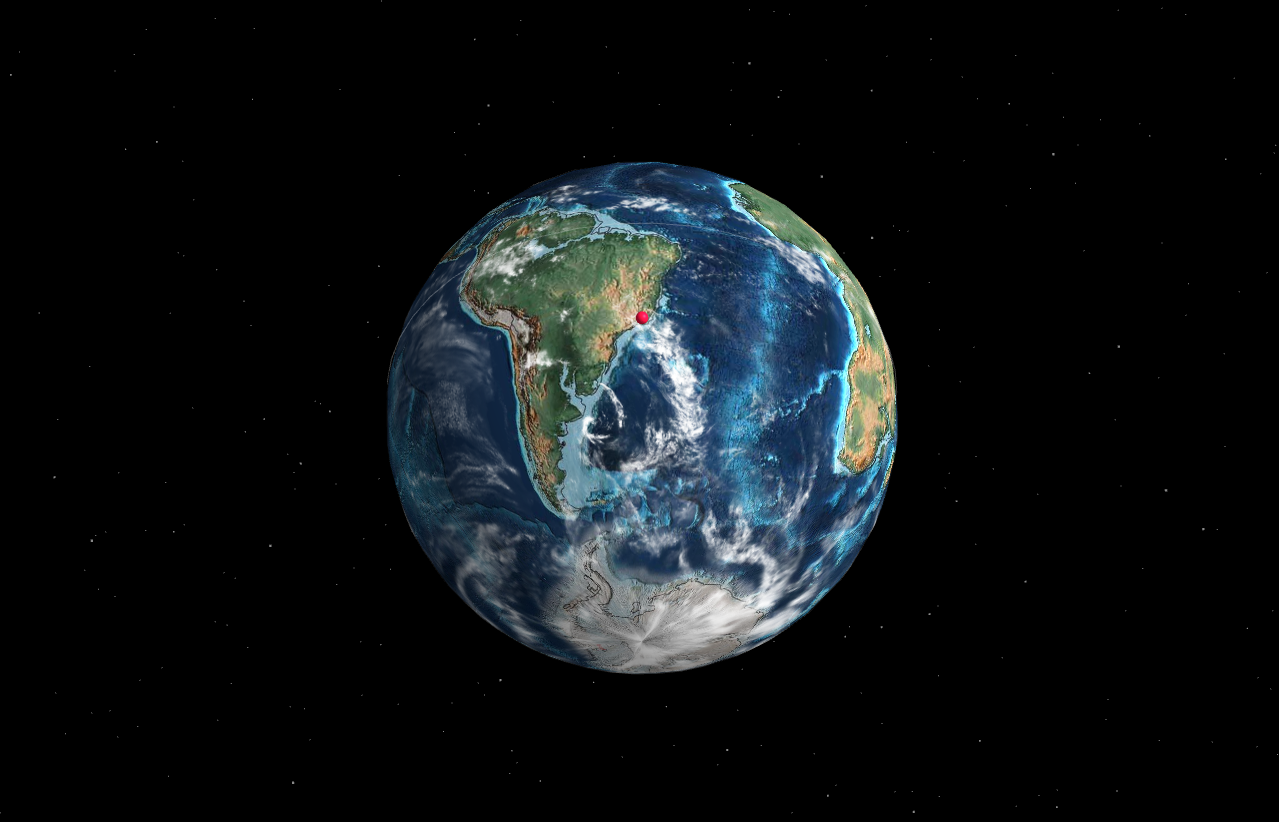
\includegraphics[width=\paperwidth,height=\paperheight]{images/neoceno.png}
	}
	
	% Frame 3: plano de fundo
	\begin{frame}
		\frametitle{\textcolor{yellow}{Agora vamos avançar bastante, no tempo ...}}
	\transdissolve	

	\flushright
    \textcolor{yellow}{$\pm$ 1.2 Ma atrás}
	\end{frame}
}


{
	\usebackgroundtemplate{
		\centering
		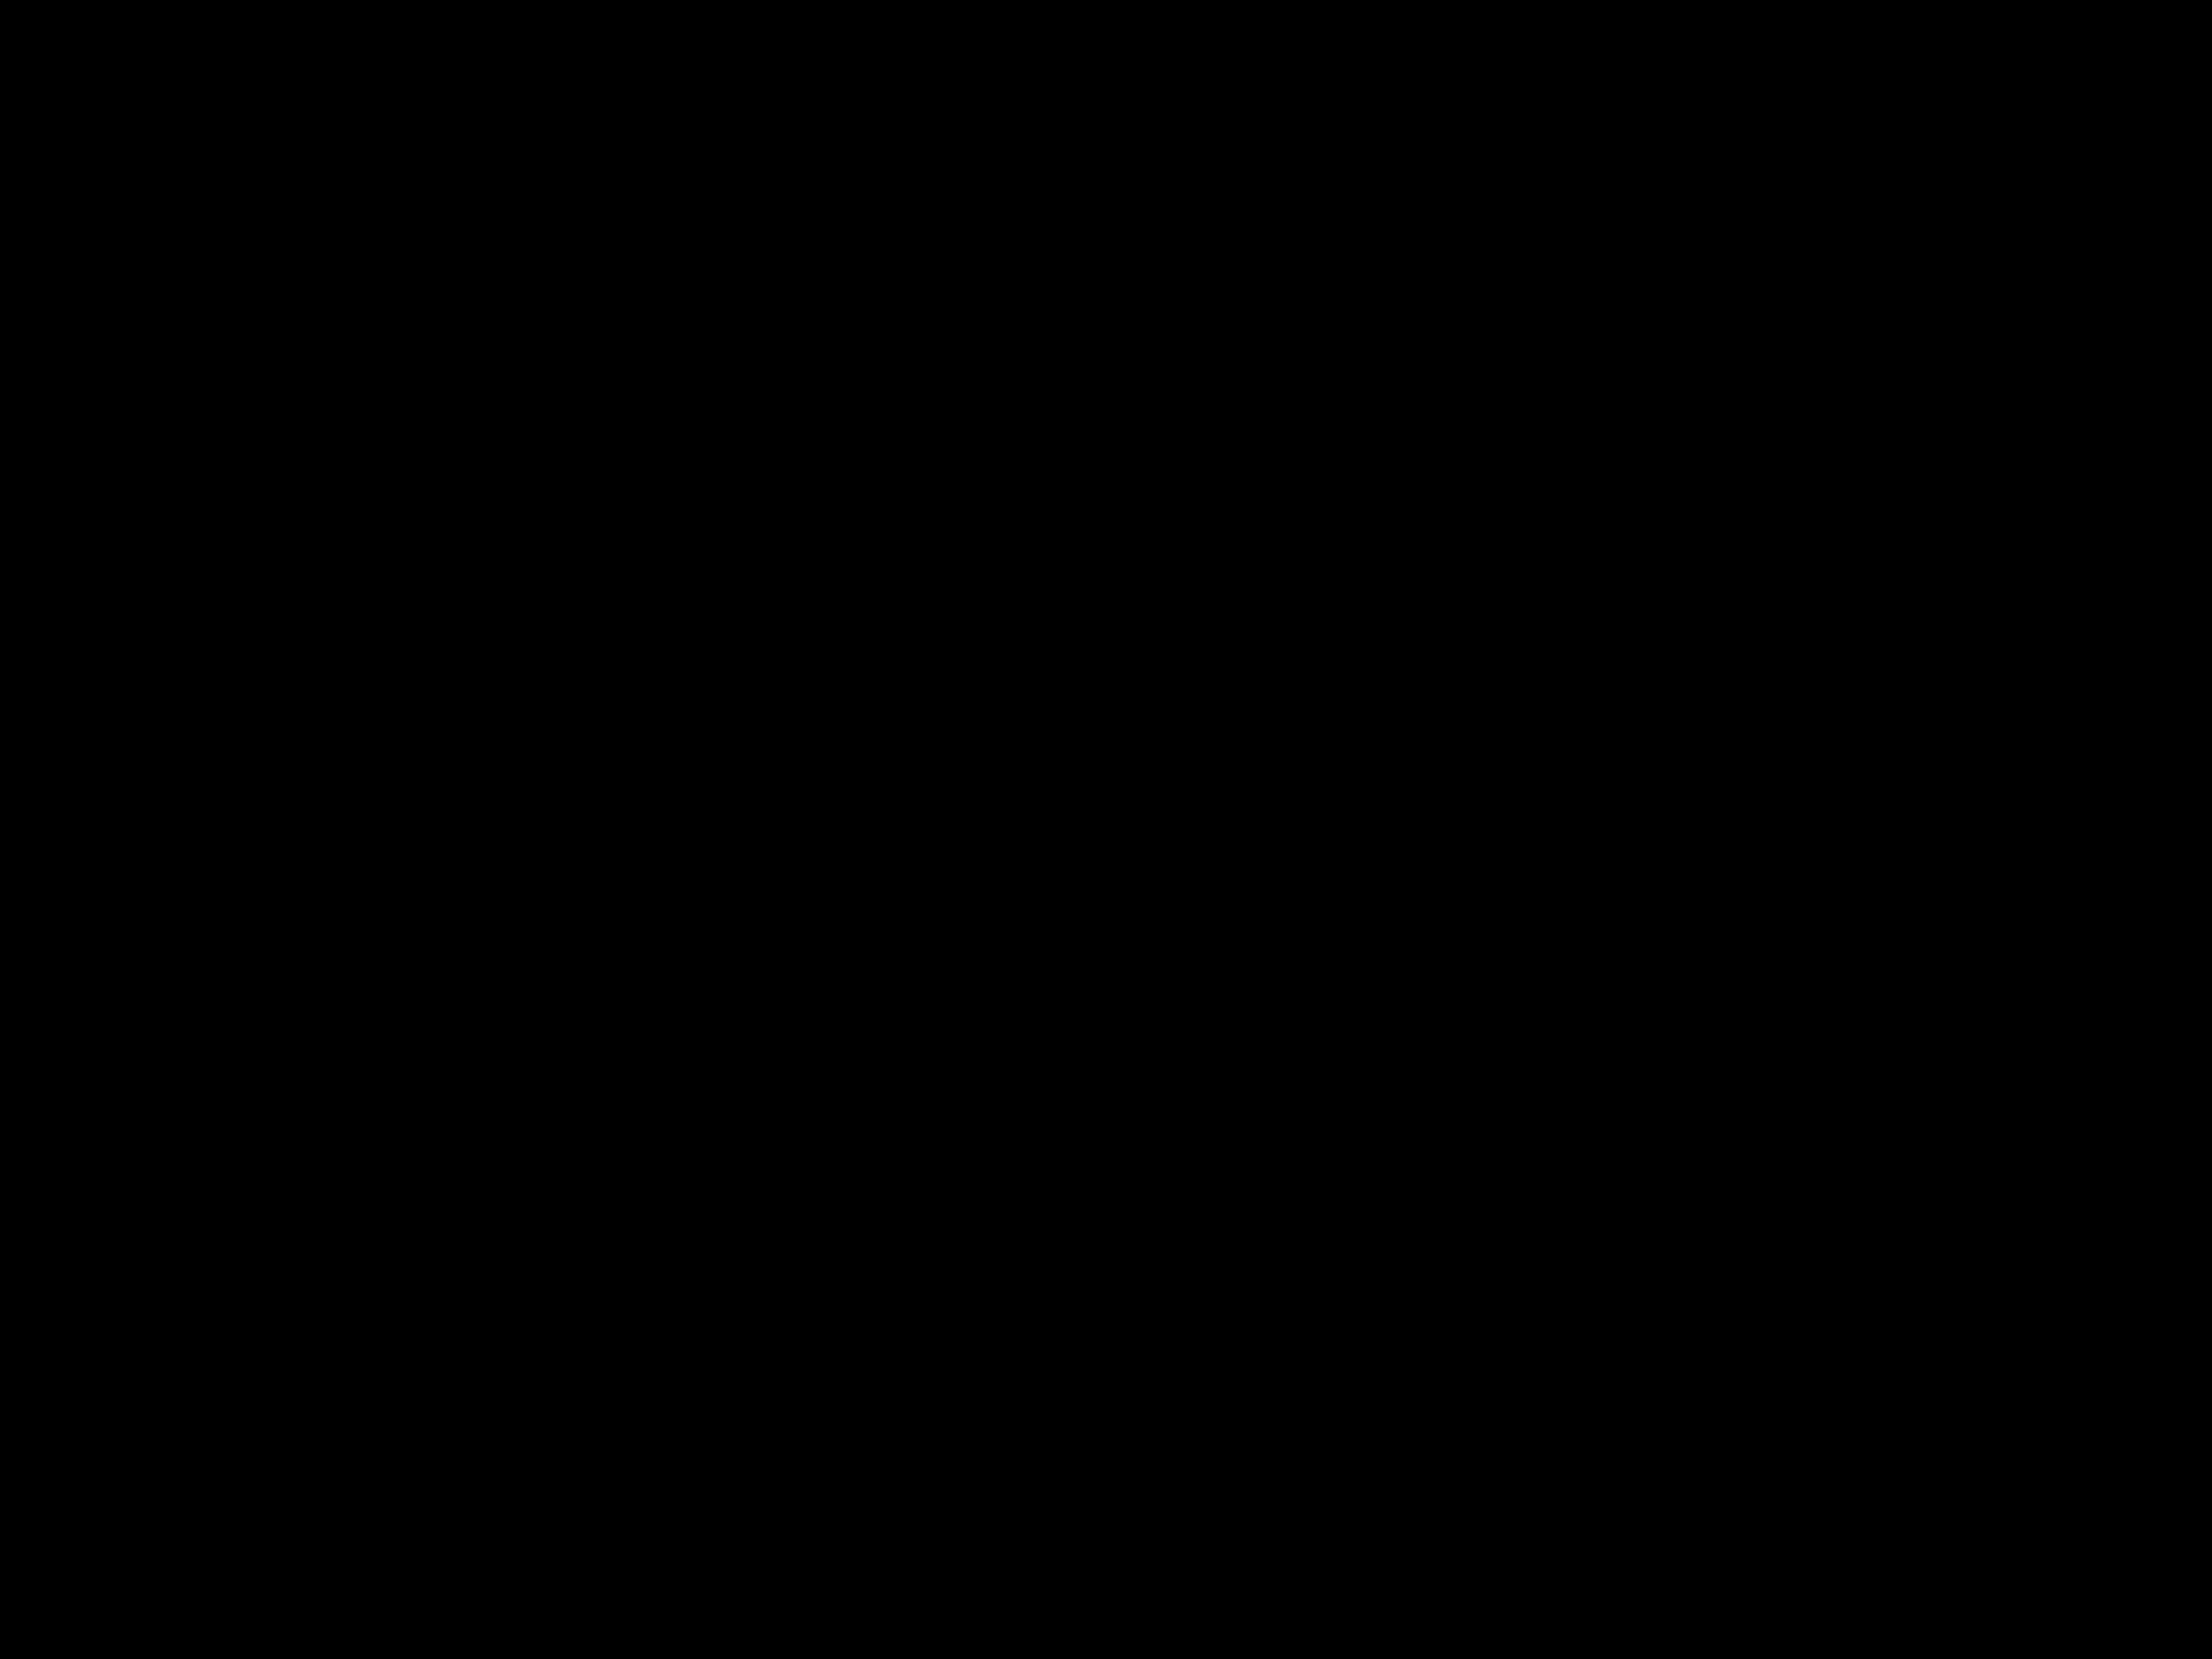
\includegraphics[width=\paperwidth,height=\paperheight]{images/fundopreto.png}
	}
	
	% Frame 3: plano de fundo
	\begin{frame}
		\frametitle{\textcolor{yellow}{Registros dos primeiros hominídeos}}
	\transboxout	
    
    \begin{minipage}{0.5\textwidth}
	    \begin{figure}
	\centering
        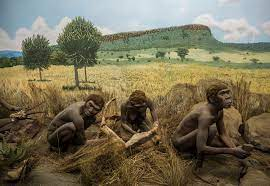
\includegraphics[scale=0.5]{images/australopitecus5.jpeg} % Substitua pelo caminho da sua primeira figura
		    \caption{\textcolor{white}{\textit{ Australopithecus afarensis}, fornece evidências sólidas do bipedismo a cerca de 3.9 Ma, na atual Etiópia.}} % Opcional
	    \end{figure}
    \end{minipage}%
		\pause
    \begin{minipage}{0.5\textwidth}
	    \begin{figure}
        \centering
        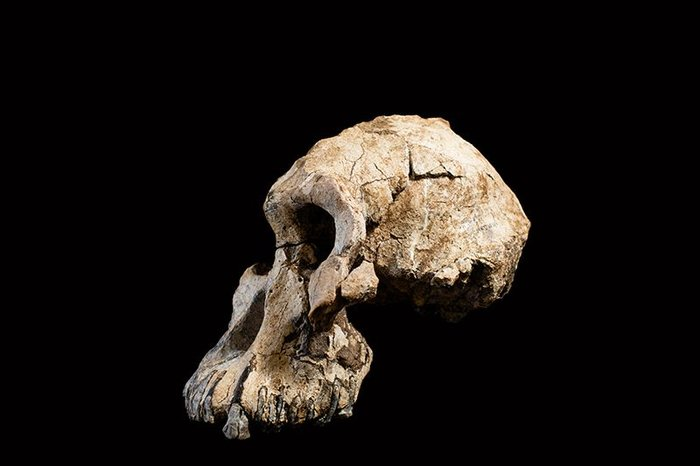
\includegraphics[scale=0.2]{images/australopitecus2.jpg} % Substitua pelo caminho da sua segunda figura
		    \caption{\textcolor{white}{Apesar de possuir andar bípede, eles tiveram braços longos. A relação do osso de braço superior (úmero) para osso de perna superior (fêmur) e está virtualmente igual ao de um Chimpanzé ($95\%$) do que um humano moderno ( $70\%$.) }} % Opcional
	    \end{figure}
    \end{minipage}

\flushright
		\textcolor{blue}{\citep{Higham2011}}
		
	\end{frame}
}




{
	\usebackgroundtemplate{
		\centering
		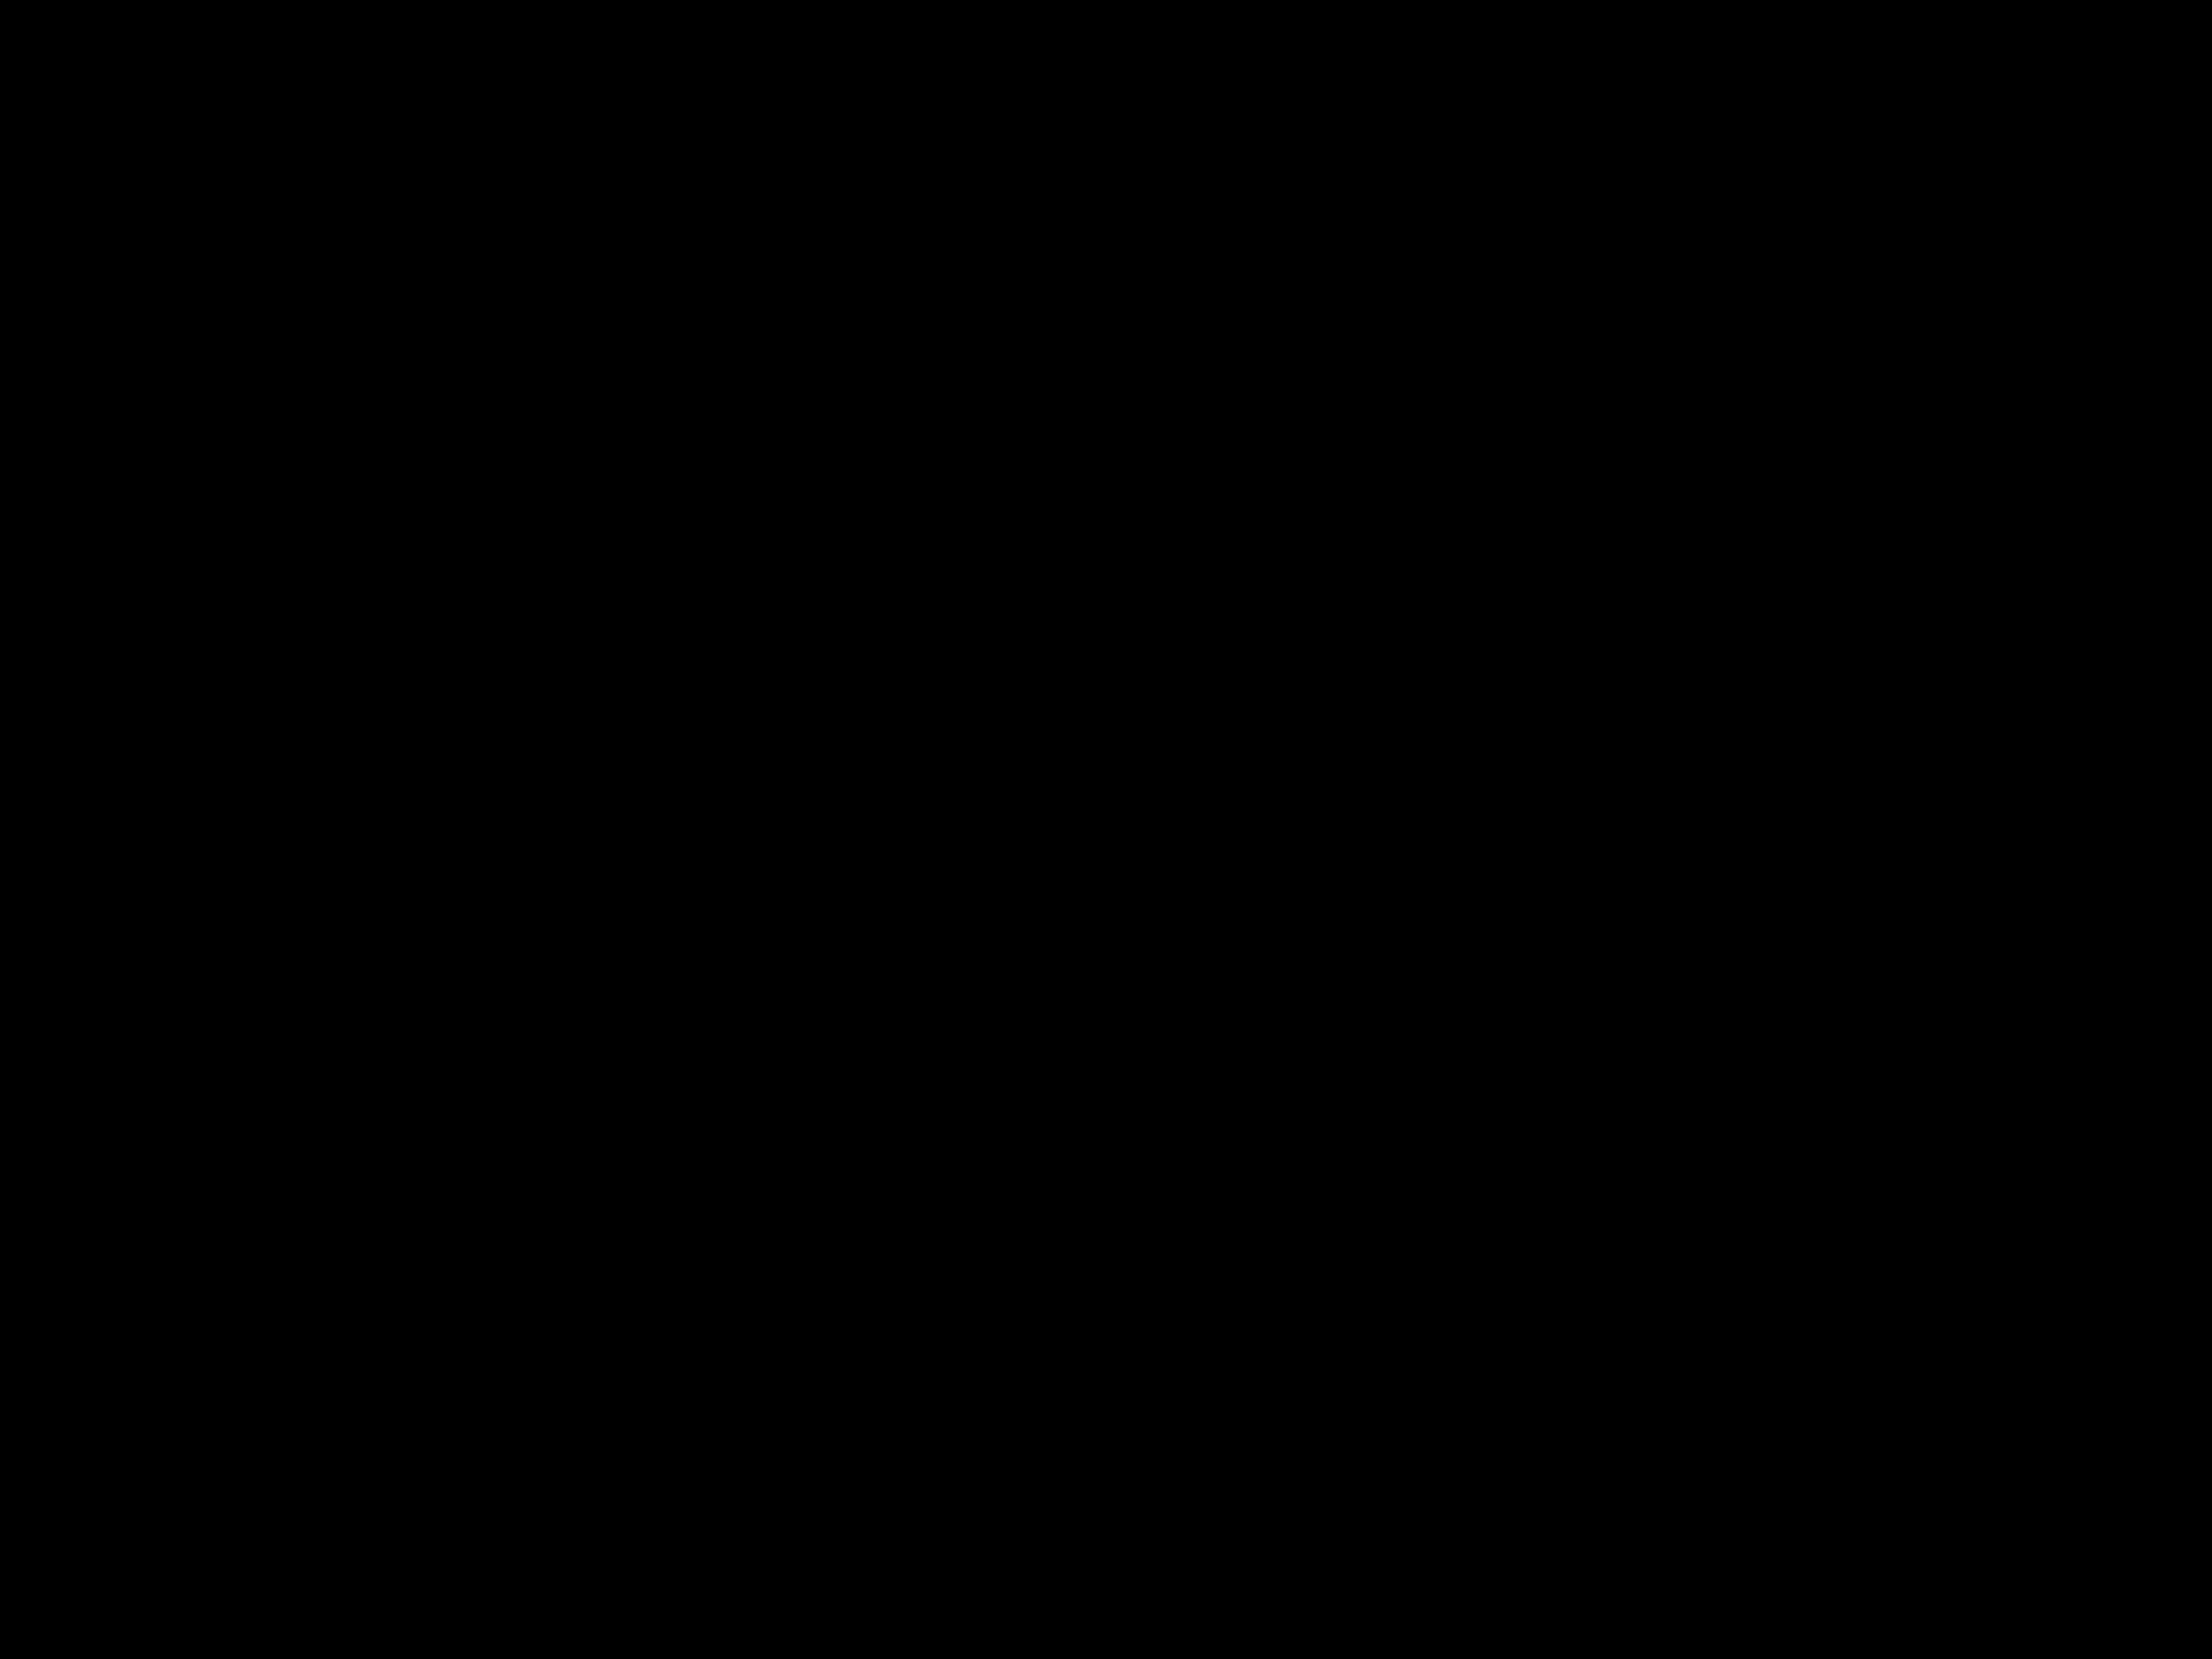
\includegraphics[width=\paperwidth,height=\paperheight]{images/fundopreto.png}
	}
	
	% Frame 3: plano de fundo
	\begin{frame}
		\frametitle{\textcolor{yellow}{Registros dos primeiros hominídeos}}
	\transboxout	
    
    \begin{minipage}{0.5\textwidth}
	    \begin{figure}
	\centering
        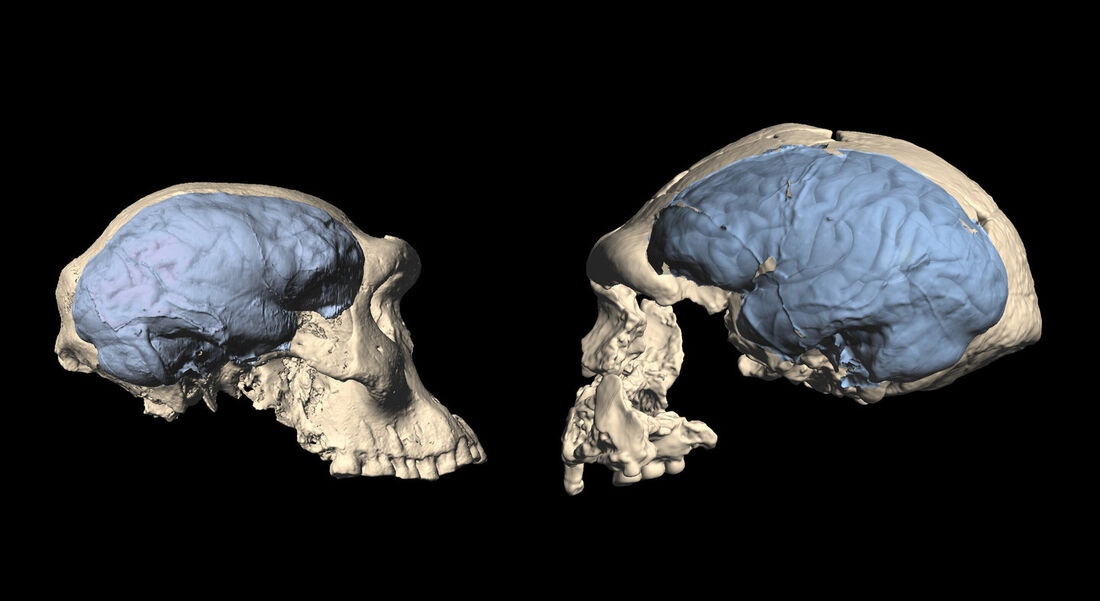
\includegraphics[scale=0.5]{images/cerebros.jpg} % Substitua pelo caminho da sua primeira figura
		    \caption{\textcolor{white}{\textit{Homo erectus}, possuía uma caixa craniana com cerca de 600 ml em média, a cerca de 1.8 Ma .}} % Opcional
	    \end{figure}
    \end{minipage}%
		\pause
    \begin{minipage}{0.5\textwidth}
	    \begin{figure}
        \centering
        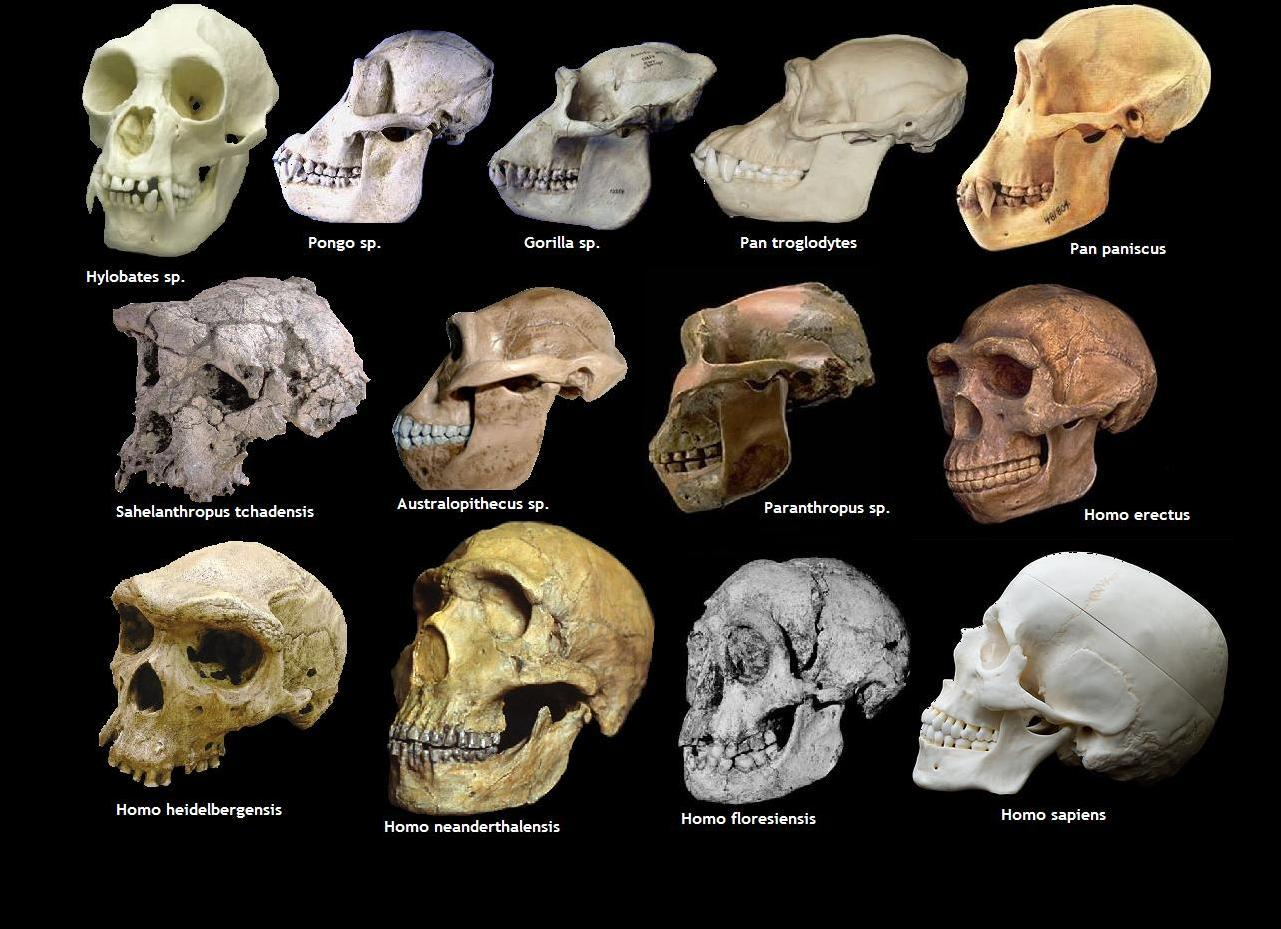
\includegraphics[scale=0.2]{images/anatomia-primata.jpg} % Substitua pelo caminho da sua segunda figura
		    \caption{\textcolor{white}{As espécies embarcam em uma marcha ascendente de crescimento cerebral, chegando a mais de 1.000 ml a cerca de 0.5 Ma. \textit{Homo sapiens} tinham cérebros com média de 1.200 ml. }} % Opcional
	    \end{figure}
    \end{minipage}

\flushright
		\textcolor{blue}{\citep{Hofman2019,Lindhout2024}}
		
	\end{frame}
}


{
	\usebackgroundtemplate{
		\centering
		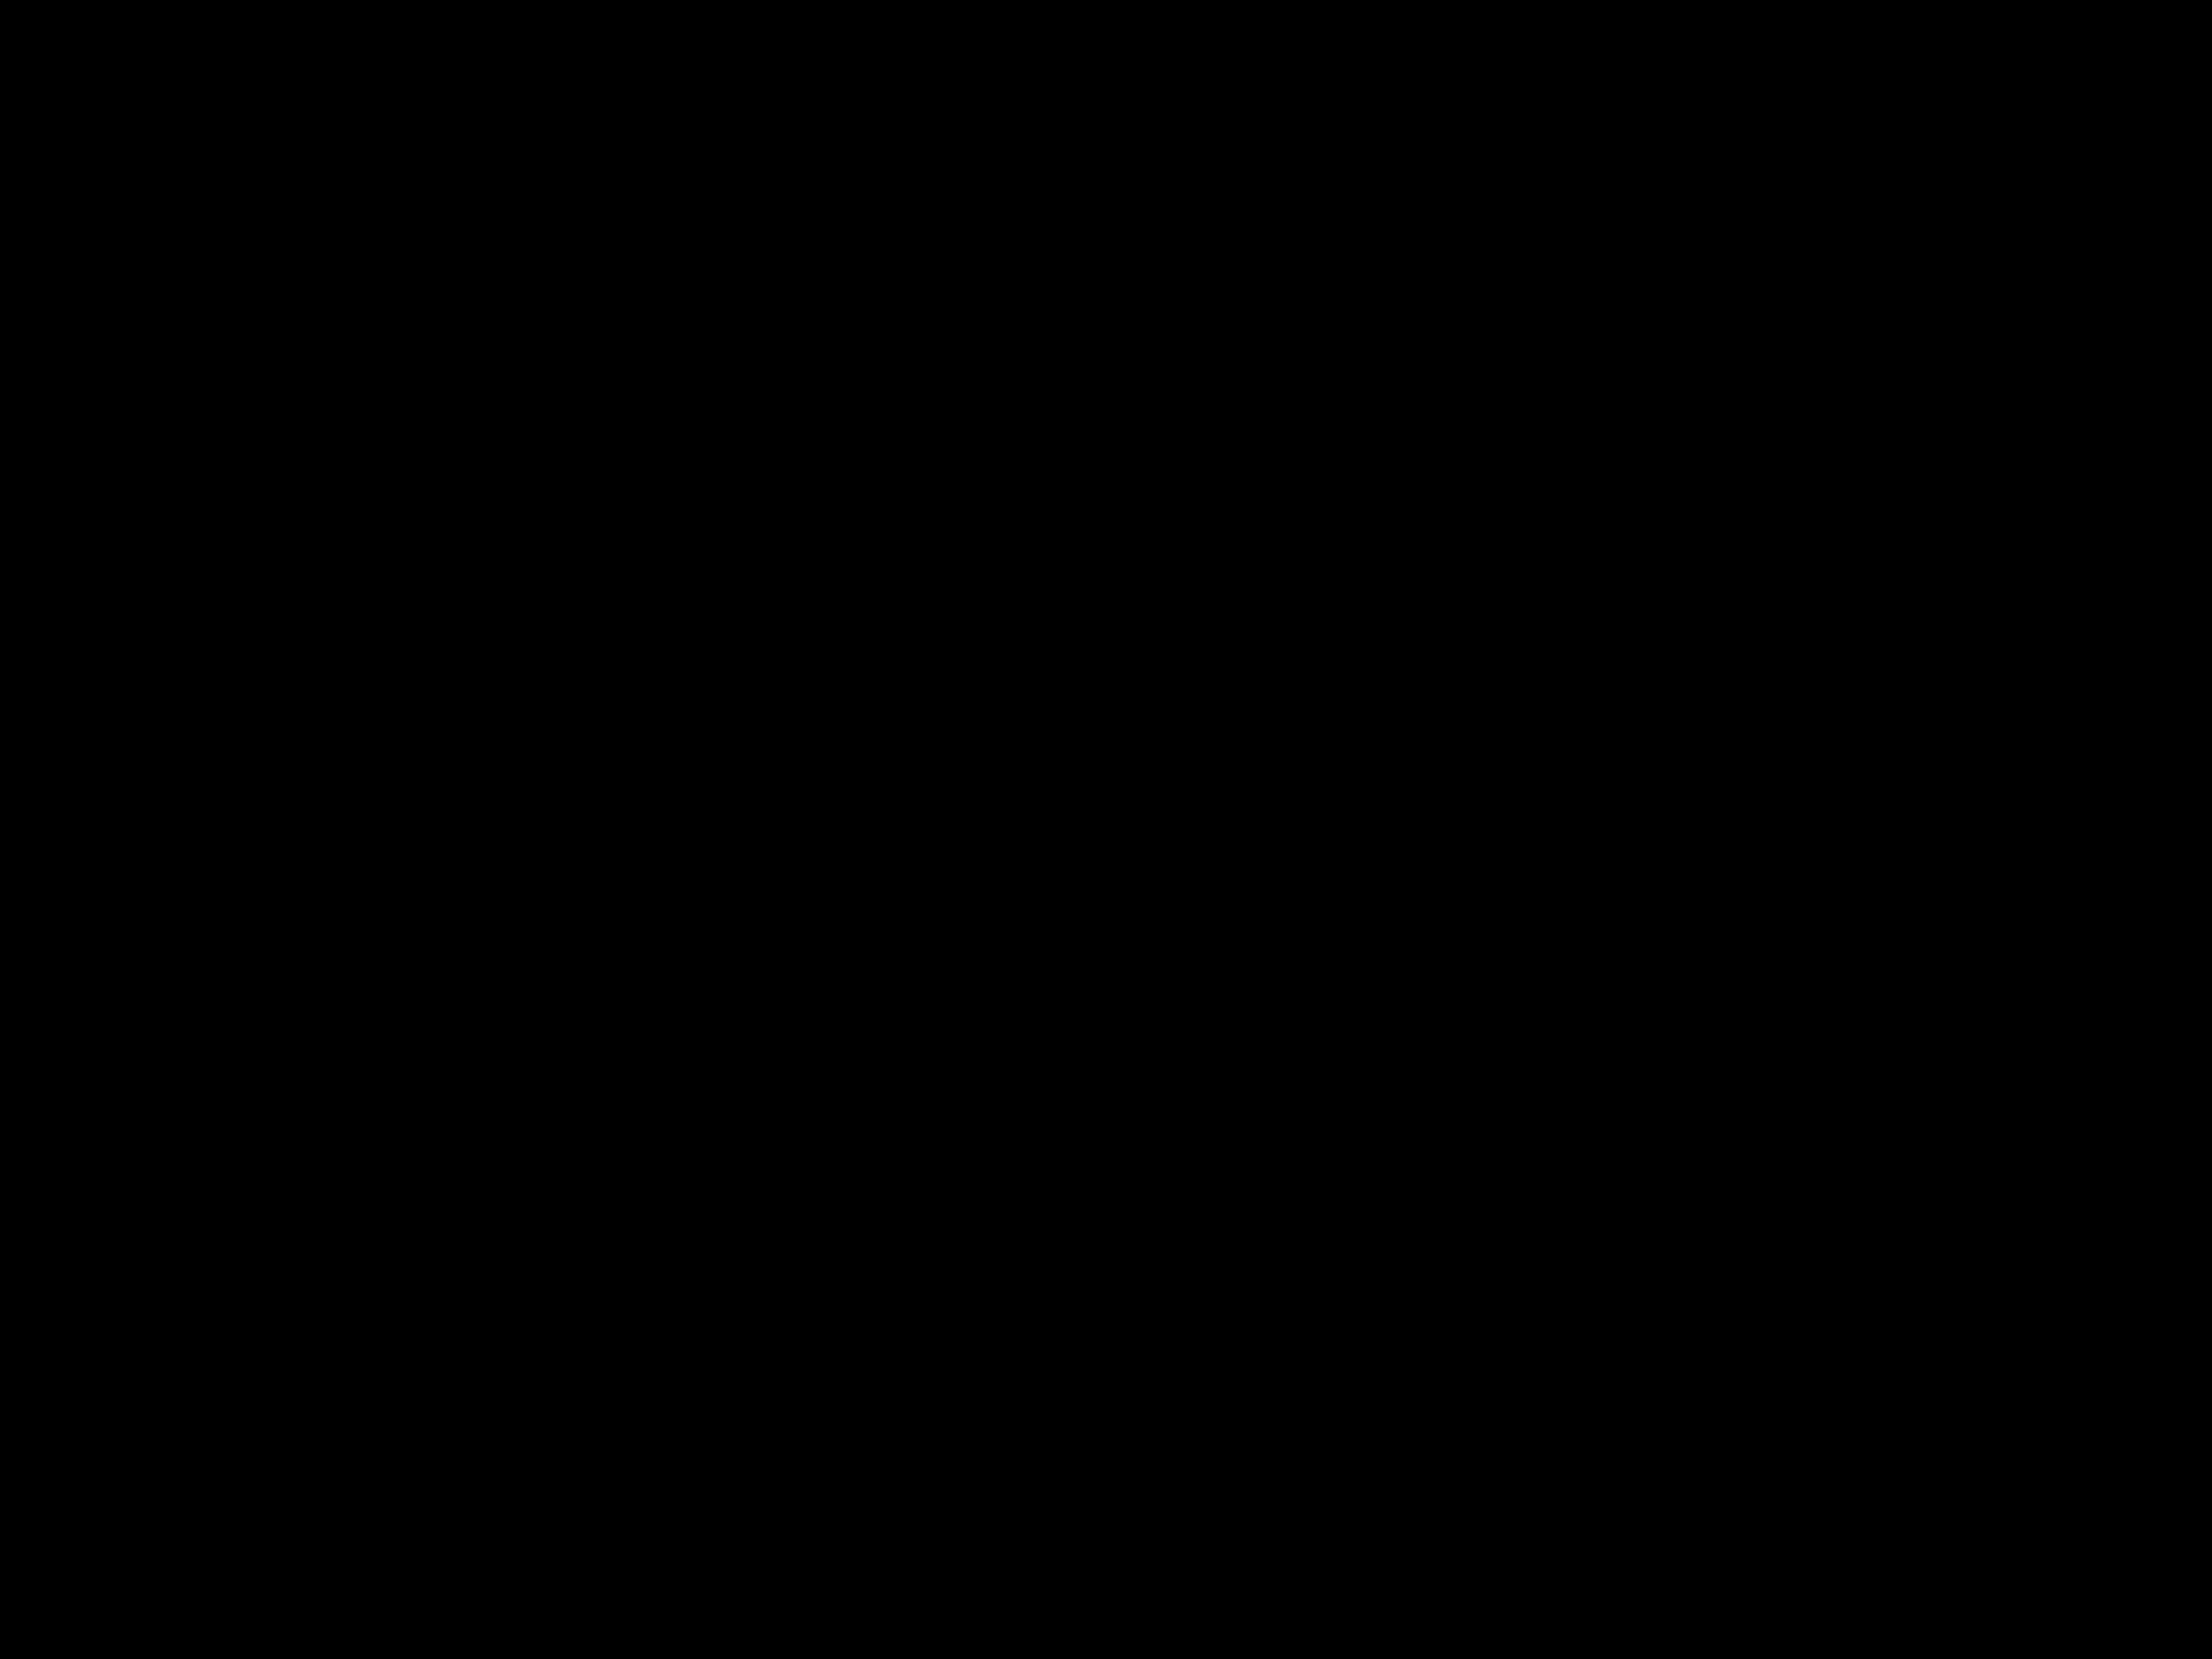
\includegraphics[width=\paperwidth,height=\paperheight]{images/fundopreto.png}
	}
	
	% Frame 3: plano de fundo
	\begin{frame}
		\frametitle{\textcolor{yellow}{O cérebro humano}}
	\transboxout	
    

	    \begin{figure}
	\centering
        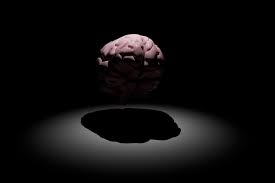
\includegraphics[scale=0.75]{images/cerebro.jpeg} % Substitua pelo caminho da sua primeira figura
		    \caption{\textcolor{white}{Composto pelo córtex cerebral (hemisférios e lobos cerebrais) e algumas estruturas profundas, como os gânglios basais, as amígdalas e o hipocampo. E as funções cerebrais supremas, como raciocinar, memorizar e prestar atenção, são controladas pelos hemisférios e os lobos que compõem o córtex.}} % Opcional
	    \end{figure}


\flushright
		\textcolor{blue}{\citep{Abbott2015,Sloan2018}}
		
	\end{frame}
}

\section{Inteligência versus aprendizado}

\begin{frame}
	\frametitle{Inteligência e aprendizado}
	\pause
	\begin{tcolorbox}[colback=gray!5,colframe=blue!40!black,title=Inteligência]
		\justifying
		\textcolor{blue}{Inteligência} é a capacidade de adquirir e aplicar conhecimento e habilidades de maneira ordenada. 
		Intellectus, que vem do verbo intelligere = dom de inteligir, entender, compreender, conhecer. Composto de dois radicais íntus = dentro e lègere = recolher, escolher.
    \end{tcolorbox}
\pause
	\begin{tcolorbox}[colback=gray!5,colframe=blue!40!black,title=Aprendizado]
		\justifying
		\textcolor{blue}{Aprendizado} é o processo de retenção de conhecimento, habilidades, valores, atitudes e competências frutos de estímulos do meio e acessados através da memória. 
		Provém do verbo apprehendere = reter, pegar, agarrar, capturar, apreender, aprender.
	\end{tcolorbox}
	\pause
	... e todo o processo pode ser modelado matematicamente tanto de forma analítica quanto em um computador.
\end{frame}


\section{Trazendo o aprendizado para um computador}


\begin{frame}
	\frametitle{Trazendo o aprendizado para um computador}
    %\pause
	%Trazer o aprendizado para um computador, requer observação e estratégia
	\begin{figure}
		\centering
		\includegraphics[scale=0.5]{images/estratégia.jpg} % Substitua pelo caminho da sua primeira figura
	\end{figure}	

	\pause

	\begin{minipage}{0.5\textwidth}
		\begin{tcolorbox}[colback=gray!5,colframe=blue!40!black,title=Estratégia 1]
			\justifying
			\textcolor{blue}{Metaheurística} é uma estratégia numérica baseada em um sorteio aleatório fruto da observação de um processo, natural ou não, que minimize uma determinada função matemática.  
		\end{tcolorbox}
    \end{minipage}%
		\pause
    \begin{minipage}{0.5\textwidth}
        \begin{itemize}
	     \item Método de Monte Carlo
	     \item Algoritmos Genéticos
	     \item Colônia de Formigas
	     \item Andar do Bêbado
	     \item Busca Harmônica
	    \end{itemize}
	\end{minipage}

\end{frame}

\begin{frame}
	\frametitle{Trazendo o aprendizado para um computador}
    %\pause
	%Trazer o aprendizado para um computador, requer observação e estratégia
	\begin{figure}
		\centering
		\includegraphics[scale=0.5]{images/estratégia.jpg} % Substitua pelo caminho da sua primeira figura
	\end{figure}	

	\pause

	\begin{minipage}{0.5\textwidth}
		\begin{tcolorbox}[colback=gray!5,colframe=blue!40!black,title=Estratégia 2]
			\justifying
			\textcolor{blue}{Métodos miméticos} conjunto de estratégias numéricas baseadas na mera observação de um processo natural, que minimize uma determinada função matemática.  
		\end{tcolorbox}
    \end{minipage}%
		\pause
    \begin{minipage}{0.5\textwidth}
        \begin{itemize}
			\item Perceptron
			\item Redes Neurais Artificiais
			\item Redes de Aprendizado Profundo
			\item Mapas Auto-organizáveis
			\item Redes de Aprendizado de Reforço
		   \end{itemize}
    \end{minipage}
\end{frame}


\section{O Perceptron e as demais RNAs}


\begin{frame}
	\frametitle{O Perceptron e as demais RNA}
	\pause
	\begin{minipage}{0.5\textwidth}
		\begin{figure}
			\centering
			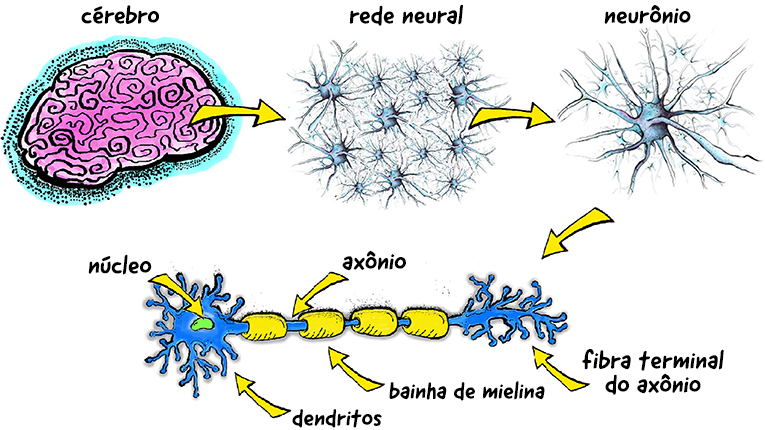
\includegraphics[scale=0.25]{images/redeneural.jpg} % Substitua pelo caminho da sua primeira figura
			\end{figure}
	\end{minipage}%
		\pause
	\begin{minipage}{0.5\textwidth}
		\begin{figure}
			\centering
			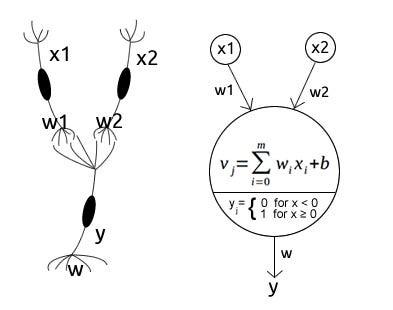
\includegraphics[scale=0.5]{images/rnxrna.jpg} % Substitua pelo caminho da sua primeira figura
			\end{figure}
	\end{minipage}
\end{frame}



\begin{frame}
	\frametitle{Um breve histórico sobre as redes neurais artificiais}
	\pause
	\begin{small}
		\smartdiagram[flow diagram:horizontal]{\textcolor{blue}{\cite{McCulloch1943}}}
	\end{small}
	\begin{itemize}
		\item Definem o a função do neurônio numérico cuja a resposta dependia da entrada dos dados da rede e dos pesos utilizados e a denominam como Perceptron.
	\end{itemize}	
\end{frame}


\begin{frame}
	\frametitle{Um breve histórico sobre as redes neurais artificiais.}
	\begin{small}
		\smartdiagram[flow diagram:horizontal]{\citet{McCulloch1943}, \textcolor{blue}{\citet{Rosenblatt1962}}}
	\end{small}
	\begin{itemize}
		\item Definem teoria de convergência do Perceptron onde ele prova que modelos de neurônios possuem propriedades similares ao cérebro humano.
	\end{itemize}
\end{frame}

\begin{frame}
	\frametitle{Um breve histórico sobre as redes neurais artificiais}
	\begin{small}
		\smartdiagram[flow diagram:horizontal]{\citet{McCulloch1943}, \citet{Rosenblatt1962}, \textcolor{blue}{\cite{Minsky1969}}}
	\end{small}
	\begin{itemize}
		\item Os Perceptrons de fato aprendem, mas somente resolvem problemas linearmente separáveis. 
	\end{itemize}
\end{frame}

\begin{frame}
	\frametitle{Um breve histórico sobre as redes neurais artificiais}
	\begin{small}
		\smartdiagram[flow diagram:horizontal]{\citet{McCulloch1943}, \citet{Rosenblatt1962}, \cite{Minsky1969}, \textcolor{blue}{\cite{Hopfield1982}}}
	\end{small}
	\begin{itemize}
		\item Resolve problemas não-lineares criando um  modelo de memória auto-associativa com a habilidade de armazenar e depois recuperar um certo conjunto de padrões do dado.  
		%\item The collective properties of this model produce a content-addressable memory which correctly yields an entire	memory from any subpart of sufficient size.
	\end{itemize}
\end{frame}

\begin{frame}
	\frametitle{Um breve histórico sobre as redes neurais artificiais}
	\begin{small}
		\smartdiagram[flow diagram:horizontal]{\citet{McCulloch1943},\citet{Rosenblatt1962}, \cite{Minsky1969}, \cite{Hopfield1982}, \textcolor{blue}{\cite{Kohonen1989}}}
	\end{small}
	\begin{itemize}
		\item Cria uma ferramenta eficiente para a identificação de padrões multivariados.  
		%\item The collective properties of this model produce a content-addressable memory which correctly yields an entire	memory from any subpart of sufficient size.
	\end{itemize}
\end{frame}



\section{Mãos à obra}

\begin{frame}
    \frametitle{Mãos à obra}
	\centering
    \href{https://playground.tensorflow.org/}{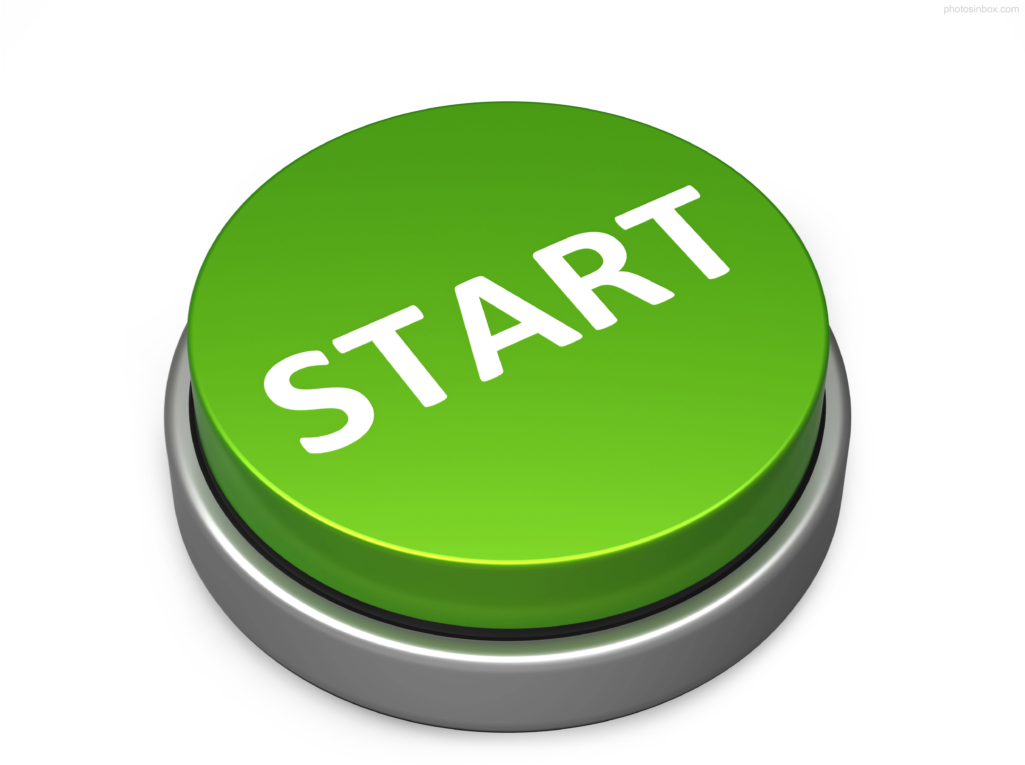
\includegraphics[scale=0.25]{images/botao.png}} 

\end{frame}




\section{Um exemplo prático}
{
\usebackgroundtemplate{
\centering
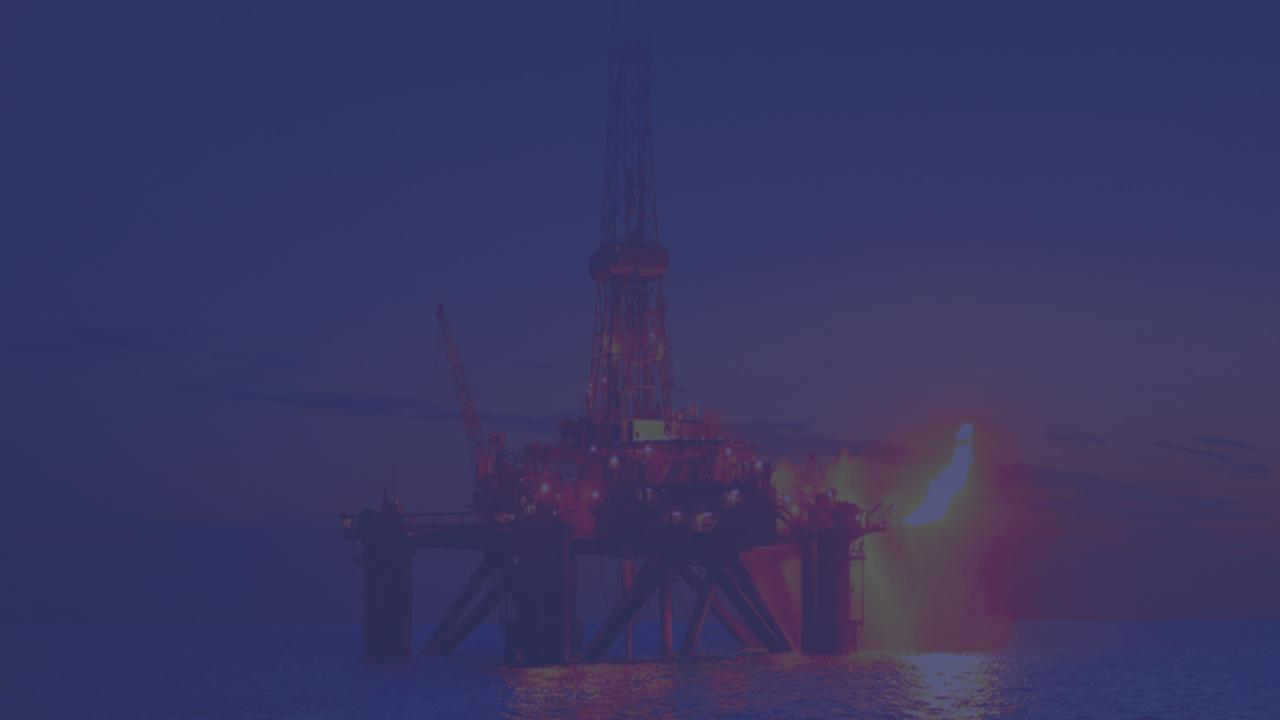
\includegraphics[width=\paperwidth,height=\paperheight]{images/fundonovo.jpg}
}
\begin{frame}
\vspace{2cm}
\begin{center}
\huge
	\textcolor{orange}{Um exemplo prático}
\end{center}

\end{frame}
}


\begin{frame}
	\frametitle{Identificação de zona de falha com dados de poços}
	\centering
	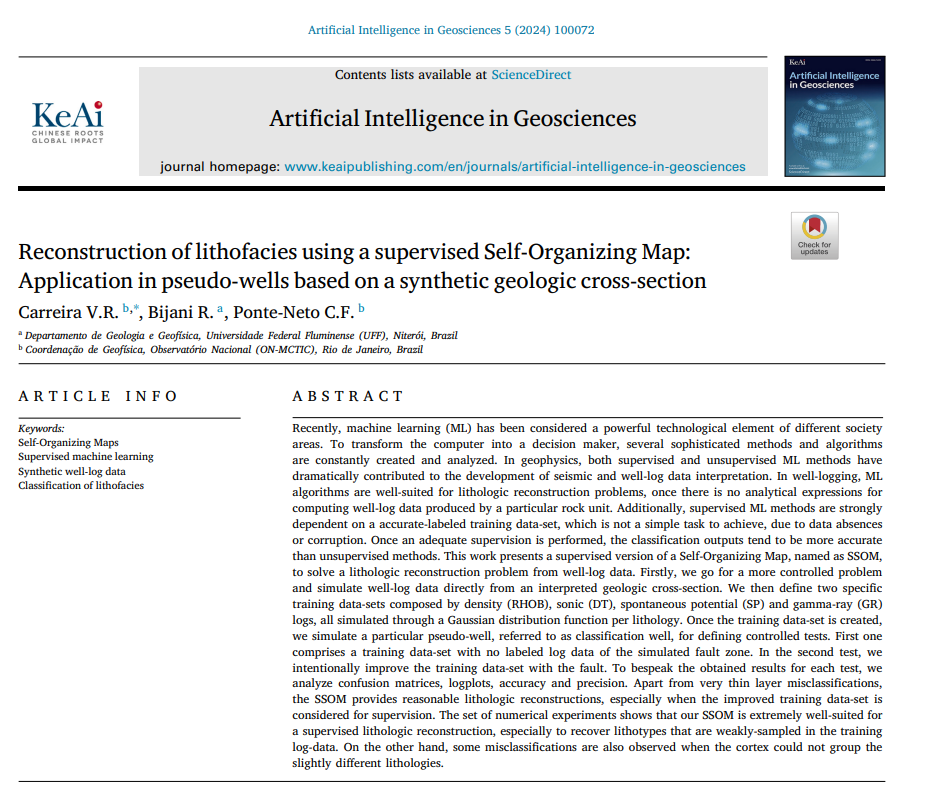
\includegraphics[scale=0.25]{images/carreira2024.png} 
\end{frame}




%
%\begin{frame}
%	\frametitle{O Mapa Auto-organizado Supervisionado}
%	\framesubtitle{Agrupamento de classes}
%	\includegraphics[scale=0.5]{images/Introkoho1.png} 
%\end{frame}
%
%
%\begin{frame}
%	\frametitle{O Mapa Auto-organizado Supervisionado}
%	\framesubtitle{Agrupamento de classes}
%	\includegraphics[scale=0.5]{images/Introkoho2.png} 
%\end{frame}
%
%
%\begin{frame}
%	\frametitle{O Mapa Auto-organizado Supervisionado}
%	\framesubtitle{Agrupamento de classes}
%	\includegraphics[scale=0.5]{images/Introkoho3.png} 
%\end{frame}
%
%
%\begin{frame}
%	\frametitle{O Mapa Auto-Organizado Supervisionado}
%	\framesubtitle{Agrupamento de classes}
%	\includegraphics[scale=0.5]{images/Introkoho4.png} 
%\end{frame}
%
%\begin{frame}
%	\frametitle{O Mapa Auto-Organizado Supervisionado}
%	\framesubtitle{Agrupamento de classes}
%	\begin{figure}
%		\centering
%		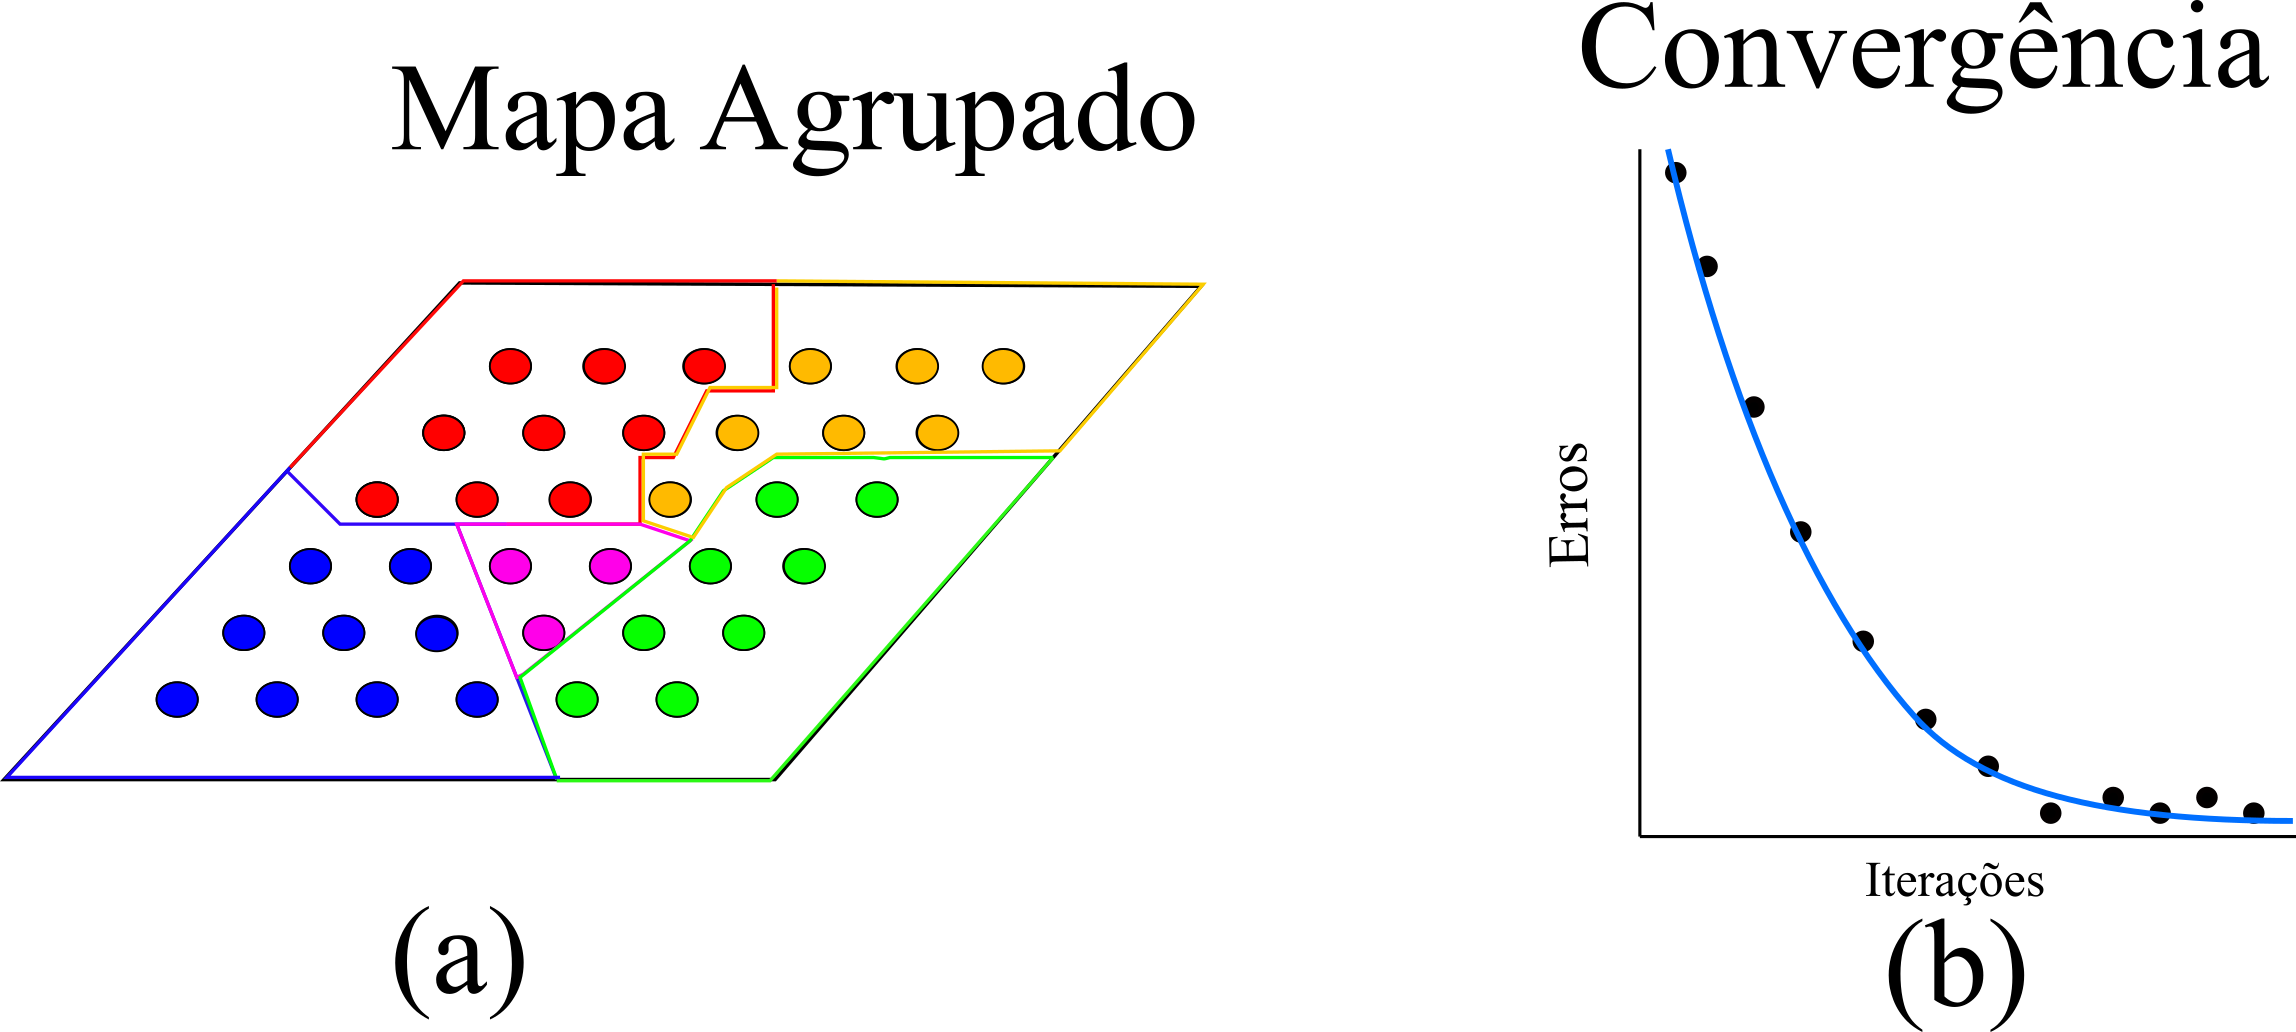
\includegraphics[scale=0.4]{images/esperadoA.png}
%	\end{figure}
%    \begin{figure}
%		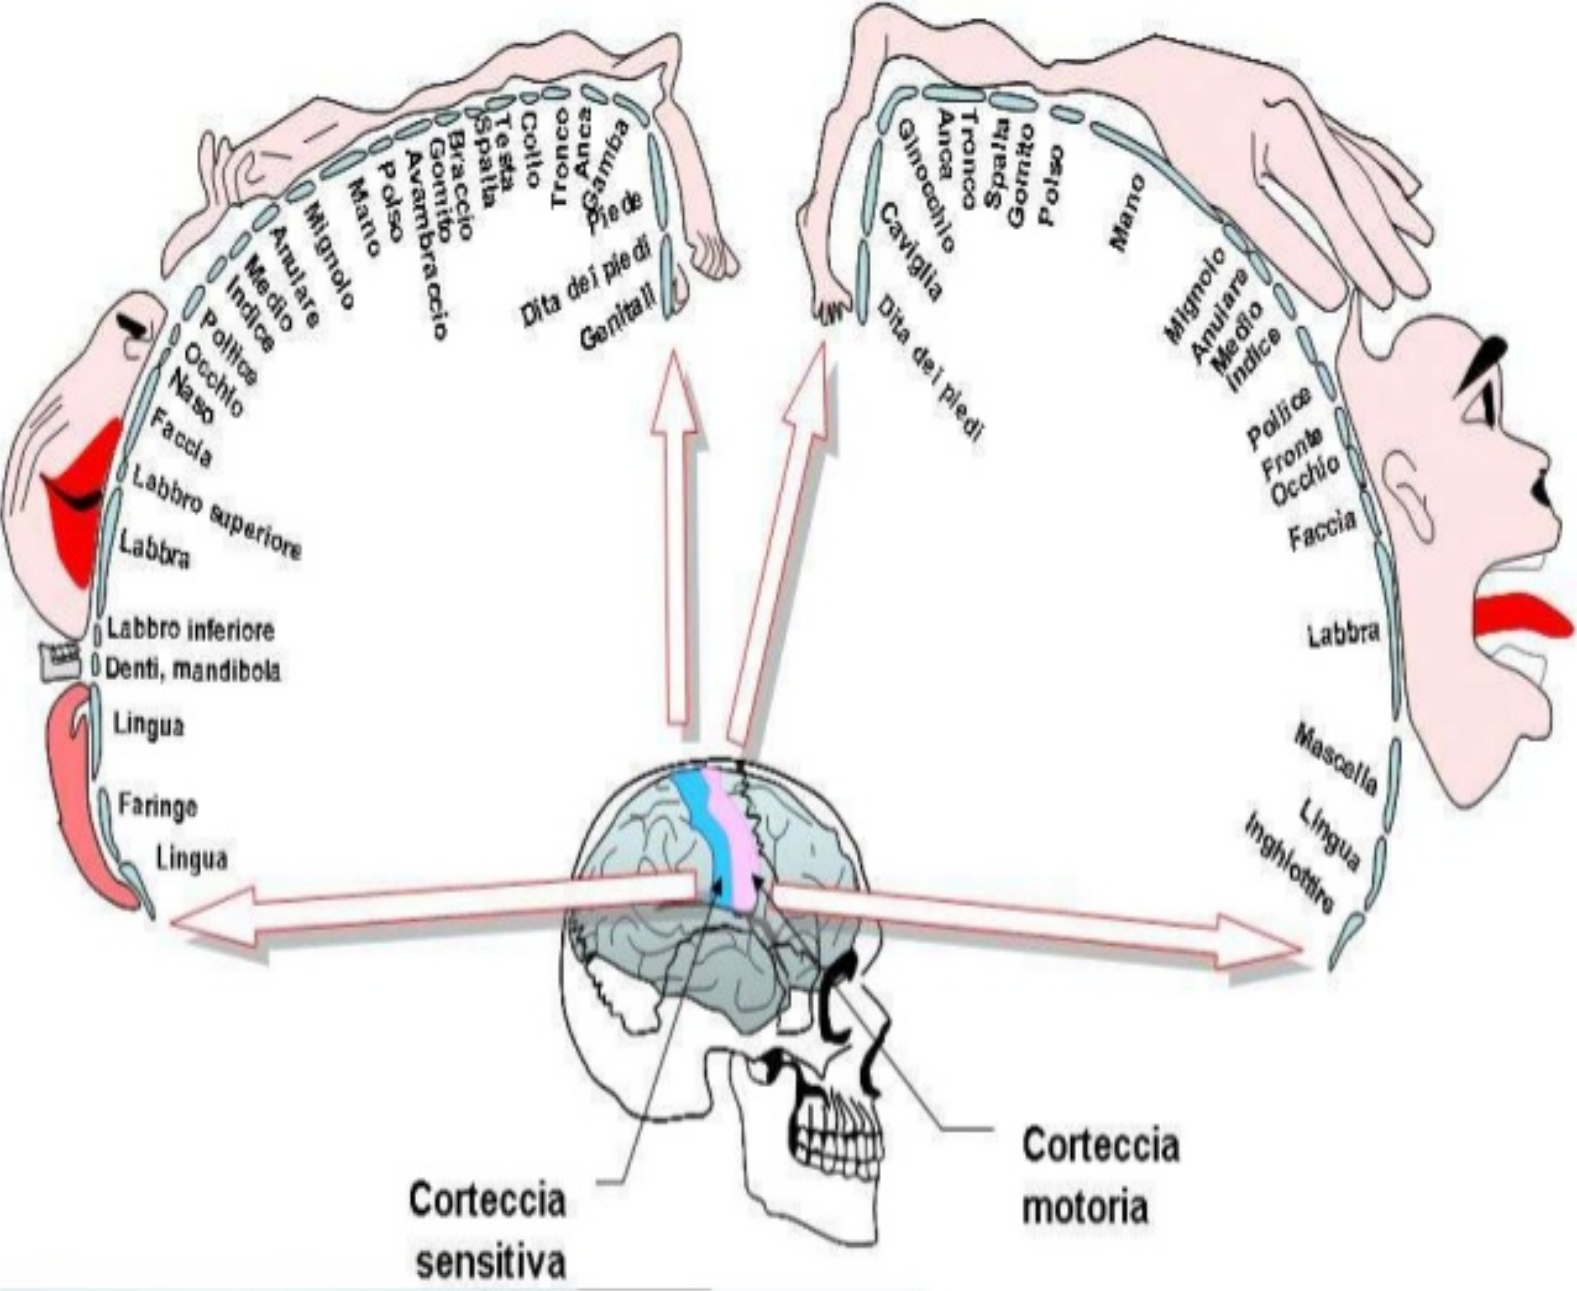
\includegraphics[scale=0.3]{images/homunculo.png}
%		\caption{\citep{Schott1993}}
%    \end{figure}
%\end{frame}























%%%%%%%%%%%%%%%%%%%%%%%%%%%%%%%%%%%%%%% REFERENCES %%%%%%%%%%%%%%%%%%%%%%%%%%%%%%%%%%%%%%%%%%%%%%%%%


{
\usebackgroundtemplate{
\centering

\includegraphics[width=\paperwidth,height=\paperheight]{images/fundo.pdf}
}
\begin{frame}[allowframebreaks]
\frametitle{Referências}
%\beamertemplatetextbibitems
\tiny
\bibliographystyle{apalike}
\bibliography{references.bib}

\end{frame}

}








{
	\usebackgroundtemplate{
		\centering
		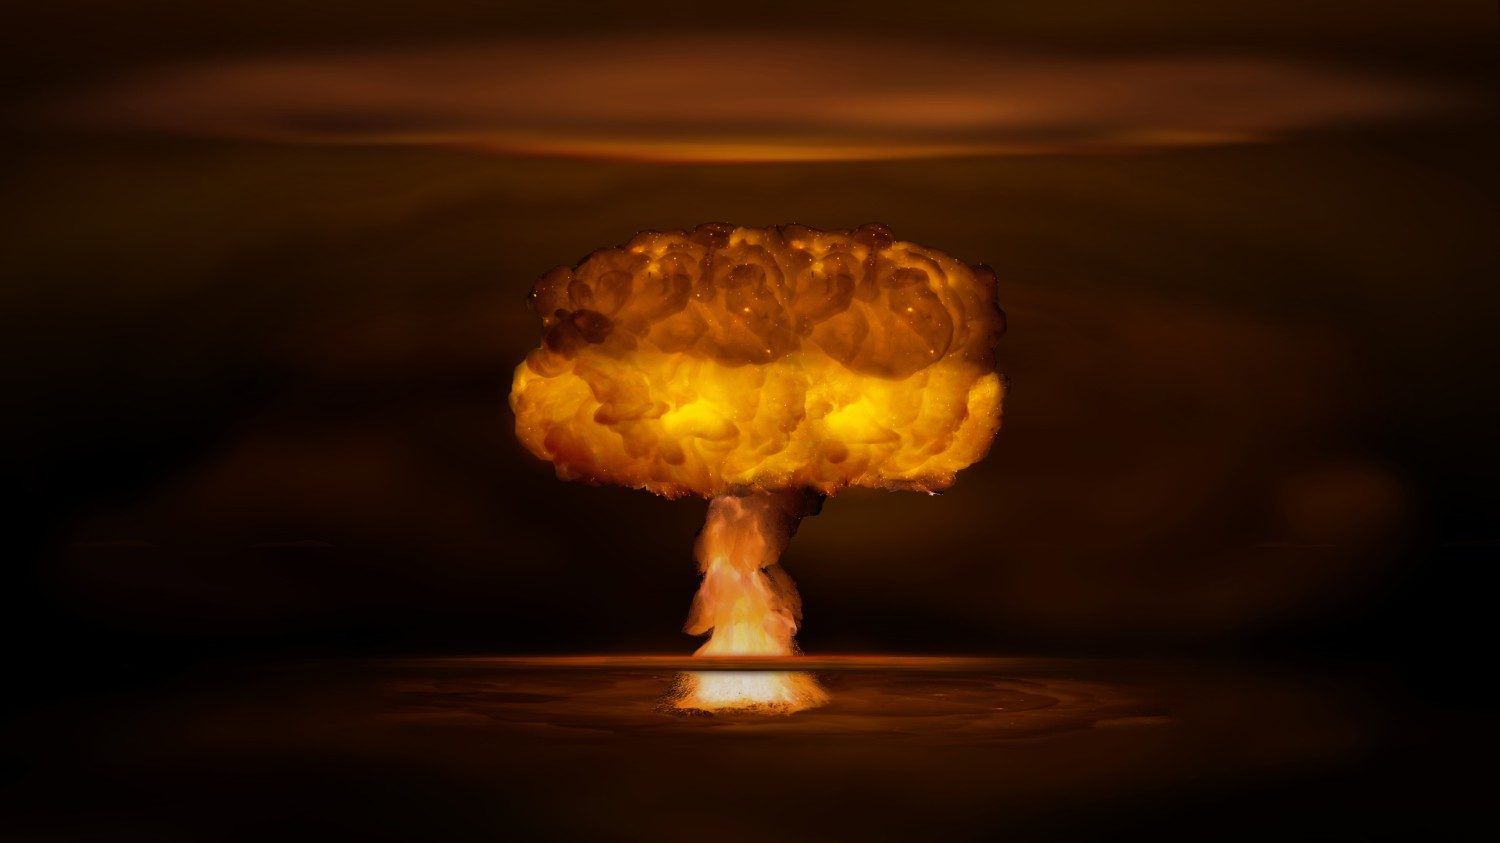
\includegraphics[width=\paperwidth,height=\paperheight]{images/bomba.jpeg}
	}
	
	% Frame 3: plano de fundo
	\begin{frame}
		\frametitle{\textcolor{yellow}{Fim}}
	



	\end{frame}
}


{
	\usebackgroundtemplate{
		\centering
		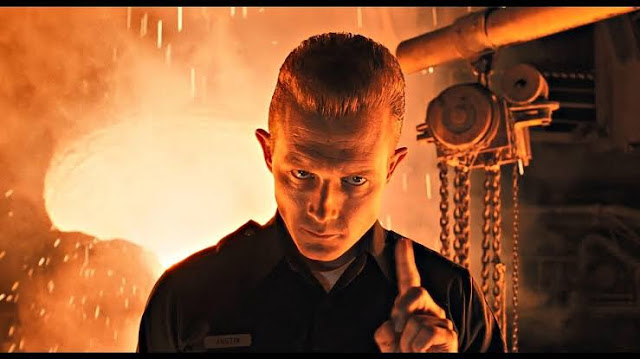
\includegraphics[width=\paperwidth,height=\paperheight]{images/terminatornao.jpg}
	}
	
	% Frame 3: plano de fundo
	\begin{frame}
	\flushright
\textcolor{yellow}{... ainda não}
	\end{frame}
}


\end{document}
